\documentclass[final]{elteikthesis}

\usepackage{booktabs} 
\usepackage{tabularx}
\usepackage{multirow}
\usepackage{makecell}


% -------- This fixes chapters ----------
\usepackage{titlesec}
\titleformat{\chapter}[hang]
  {\normalfont\huge\bfseries}
  {\thechapter.} 
  {1em}
  {}
% -------- This fixes margins -----------
\usepackage{geometry}
\geometry{
  left=25mm,
  right=25mm,
  top=25mm,
  bottom=25mm
}
% ---------------------------------------

% -------- Paragraph spacing control ----
\setlength{\parindent}{6pt}
% ---------------------------------------


\addbibresource{references.bib}

\title{EEG Artifact Detection and Filtering Using Machine Learning and Deep Learning Approaches}
\date{2026}

\author{Benjámin Tóth}
\degree{Computer Science MSc}

\supervisor{László Gulyás}
\affiliation{Associate Professor, PhD}

\extsupervisor{András Lukács}
\extaffiliation{Associate Professor, PhD}

\university{Eötvös Loránd University}
\faculty{Faculty of Informatics}
\department{Department of Artificial Intelligence}
\city{Budapest}

\logo{elte_cimer_szines}

\begin{document}

\documentlang{english}

\maketitle

\begin{abstract}

Artifacts in electroencephalography (EEG) hinder automated analysis, particularly in seizure detection. While EEG data are costly to label at scale, modern generative models can synthesise realistic, label-aware artifact segments suitable for augmentation. A latent diffusion-based augmentation method with a per-class training strategy is proposed to improve artifact classification performance in imbalanced settings. To address class imbalance, the training data is extended with synthetic EEG signal segments, improving data diversity and class representation. Using the TUH EEG Artifact (TUAR) corpus, the proposed method is evaluated and compared against existing non-generative and generative augmentation techniques. Results show that latent diffusion-based augmentation improves artifact classification by 3.7\% in Macro F1 and 3.5\% in Macro PR AUC and demonstrates small but consistent improvements when combined with existing augmentation pipelines. Although the proposed method is not able to outperform all baseline approaches, it demonstrates consistent improvements in classification performance and showcases the potential of latent diffusion-based augmentation for imbalanced EEG artifact datasets. 

\end{abstract}
\chapter*{Acknowledgements}

I would like to express my gratitude to my internal supervisor Professor László Gulyás for his valuable insights and guidance throughout this thesis. I would also like to thank my external supervisor Professor András Lukács for providing professional guidance and necessary tools for this study. I am also grateful to the Institute of Mathematics for providing server access and GPU resources.


\newpage

\tableofcontents

\chapter{Introduction}

\section{Motivation}

Electroencephalography (EEG) is one of the most commonly used techniques for measuring brain activity. This technique finds application not only in clinical settings but also in research into neurology. However, EEG techniques that are used in practice are very sensitive to artifacts originating from the position of the electrodes and physiological electrical noise. 

These artifacts are able to corrupt the signal, which makes interpretation and EEG analysis significantly more difficult. Epilepsy or seizure detection, anesthesia depth monitoring and emotion recognition are fields that are often corrupted by artifacts similar to meaningful neural activity. This can often produce false positives and often results in degraded model performance.

With the application of EEG classification methods, misinterpretation of brain activity can be significantly reduced. Modern deep learning models demonstrate great results in solving such tasks as they are capable of learning complex signal characteristics of raw EEG data. These methods demonstrated state-of-the-art performance on many EEG classification benchmarks and become a basic tool in both clinical and research applications.

The main weakness of deep learning approaches is their requirement of large amounts of labeled data. EEG dataset annotation is expensive, time-consuming, and requires trained experts to accurately classify recordings, which results in their limited availability. Another problem is that the occurrence of different types of artifacts varies strongly in EEG recordings. This results in class imbalance, where rare labels are underrepresented while major artifacts dominate.

In order to over these challenges in the field, new methods are needed to improve data efficiency and boost model generalisation without requiring additional manual annotation.

\section{Why Generative Augmentation}

Data augmentation techniques offer solution to data scarcity and help improve generalisation. There are traditional augmentations used for EEG data, similar to the image based augmentation methods, such as noise injection, shifting, and cropping. There are also EEG specific methods including channel dropout, frequency and time-domain augmentations.

Generative augmentations also demonstrated strong results by extending existing datasets with fully synthetic data. This data is produced by generative models capable of learning the statistics of the original dataset and producing synthetic datapoints from the estimated distribution. The best results are often achieved by a combined augmentation pipeline, in which the synthetic data is generated and added to the dataset, then the traditional augmentations are applied, further increasing data variance.

Generative adversarial networks are widely used for dataset expansion, achieving performance gains in most pipelines. Diffusion models offer a powerful alternative that presents more stable and consistent training behavior with the technique of gradually transforming noise into realistic samples. 
Latent diffusion is a variant of the diffusion model family in which the generative process takes place in a compressed latent space with reduced computational complexity. This solution is also advantageous for high-dimensional EEG data.

While these models become popular in most deep learning frameworks, the application of latent diffusion methods to EEG artifact augmentation remains limited. This thesis addresses this gap by investigating the effectiveness of a proposed latent diffusion-based augmentation method in comparison with other augmentation techniques.

\section{Contributions}

The main contribution of this thesis is a latent diffusion-based augmentation method, specialised for synthetic EEG artifact generation in imbalanced datasets. A per-class augmentation strategy is introduced in this work, in which a separate model is trained for each class and evaluated using the TUAR dataset for artifact classification.

A comprehensive comparison is conducted and analysed in this study, where the proposed augmentation method is compared to commonly used nongenerative baseline augmentations and a WGAN-based generative model. The effects of the augmentations are evaluated on a diverse set of EEG classification models, including baseline and state-of-the-art architectures. In the first experiment, all model-augmentation pairs are trained multiple times to compare the effects of different augmentation methods to the proposed method. In the second experiment the effect of proposed technique is measured when it is applied together with existing augmentation pipelines, and compared to their baseline performance. The results demonstrate that the proposed latent diffusion-based approach can improve classification performance.

This study also focuses on the imbalanced aspect of artifact detection by analysing improvements separately for each class. It demonstrates that the synthetic EEG data generated using the latent diffusion model can improve classification performance for both dominant and underrepresented classes.

Additionally, the thesis provides a detailed description of the implemented preprocessing pipeline and a clinically realistic dataset splitting technique, which are particularly important in the field of EEG classification and for the reproducibility of the experimental results.

\chapter{Background}
\label{chap:background}

\section{Related Work}

\subsection{EEG Classification Methods}

A wide range of methods have been proposed to detect patterns in brain activity corresponding to health related events, cognitive activities, and specific mental states. The goal of these methods is to extract information from raw EEG signals corresponding to high-level brain states, which enables advanced diagnostic techniques, monitoring, and brain–computer interfaces.

Classical machine learning algorithms formed the basis of early EEG classification systems combined with manually designed feature extraction pipelines \cite{8972542}. These methods apply traditional classifiers to the extracted features, such as k-nearest neighbors, naive Bayes, support vector machines, decision trees, and random forests \cite{technologies10040079}. The main problem with these models is their dependence on feature extraction quality and their limited generalisation ability to larger datasets.

Deep learning-based classification methods have become popular in recent years. The most commonly used model family in the industry is convolutional neural networks (CNNs), which use temporal and spatial convolutions, as in EEGNet \cite{Lawhern_2018}, ShallowFBCSPNet \cite{EEGInceptionERP}, and EEGInceptionERP \cite{EEG-Inception}. Purely CNN models like EEGNeX \cite{CHEN2024105475} are still able to achieve SOTA performance on many benchmark problems. 

Recurrent neural networks (RNNs) combined with CNNs are able to both learn spatial feature extraction and perform sequence modeling. Hybrid CNN-LSTM \cite{inproceedings} models provide strong foundation and enable improved classification performance. 

Attention-based models further improve EEG analysis with the ability to capture long-range dependencies. Architectures like EEGConformer \cite{Conformer} and EEGPT \cite{wang2024eegpt} have delivered promising results in classification tasks where temporal patterns play a significant role.

The introduction of graph neural networks (GNNs) has also gained attention in the field, but these methods are still relatively new, and their effectiveness and applicability remain not fully established.

Despite the strong results of deep learning-based methods, their performance highly depends on the amount of labeled data, making classical machine learning approaches remain competitive in many real-world scenarios.

\subsection{EEG Artifact Detection}

EEG recordings often contain artifacts, which are characteristic signal patterns corresponding to different sources. Some earlier works focused on the suppression or removal of these artifacts, mainly by using filtering techniques \cite{QUAZI2017401} and developing strong preprocessing pipelines \cite{RICOOLARTE2025103702}. Recent studies even apply deep learning techniques on synthetic and real datasets with the goal of complete artifact removal \cite{FERNANDEZDERETANA2025152}\cite{app15094953}.

Deep learning techniques become SOTA solutions for classification tasks defined by benchmark artifact datasets. The TUH EEG Artifact Corpus (TUAR) \cite{9353647} provides large number of EEG recordings on which many models and methods are tested. There are earlier works that introduce both single label and multi label classification setups using the TUAR dataset \cite{TUAR}.

Studies have built upon the TUAR benchmark, developing new models \cite{TUAR2} and exploring energy-efficient monitoring techniques for epilepsy detection \cite{energy}, yet relatively few works have focused on classifying rare artifacts and solving challenges caused by class imbalance.

Additionally, artifacts are also explored with the aim of improving seizure detection models \cite{inproceedings}, due to the temporal and morphological similarities of seizure and certain artifact characteristics, while other studies focus on data splitting techniques to simulate realistic clinical environments.

\subsection{Data Augmentation Techniques}

The introduction of deep learning techniques and their success in EEG related tasks has shifted the focus to data augmentation techniques. Due to the large data requirements of these models, augmentations that increase the variance of the dataset have proven useful for problems with low samples-to-features ratio \cite{LASHGARI2020108885}.

Some works evaluate the effects of specific augmentation methods, such as pink and Gaussian noise addition \cite{pink} or time–frequency transformations \cite{WANG2025113074}, while others focus on developing stronger data augmentation pipelines for a targeted use case like epilepsy detection \cite{epi}. These solutions have become an essential component of most EEG related deep learning approaches. 

In recent years, generative models proved to be the next step in the field of EEG augmentation as well by introducing fully synthetic data generation techniques. Using generated data not only increases variance in the dataset, but also helps address data imbalance problems. Recent works have successfully improved overall performance with class specific data generation \cite{Fan_2020}.

Most studies have used generative adversarial networks (GANs) for data generation \cite{gan2}, but diffusion-based methods have emerged as a new candidate for such tasks \cite{puah2025}. Both models have been used in many studies for enhancing and expanding existing smaller datasets, while relatively few have focused on artifact specific data generation.

A related study compared GAN and diffusion models for EEG artifact synthesis, but its main objective was to evaluate class-conditional consistency rather than to improve classification performance using the generated data, and the diffusion model operates directly on the raw signal instead of a latent space \cite{arasu2025}.

While recent works highlight growing importance of data oriented approaches in EEG analysis, they also present a gap in the systematic evaluation of augmentation strategies for artifact classification tasks.

\newpage

\section{Dataset}

\subsection{TUAR Dataset Description}

The dataset used was the TUH EEG Artifact Corpus (TUAR) \cite{9353647}. This dataset is a subset of the Temple University Hospital EEG Corpus (TUH EEG), a large-scale collection of clinical EEG recordings gathered during routine patient care at Temple University Hospital. The TUH EEG dataset was created to support research in machine learning and deep learning methods, EEG analysis and classification. TUAR is a specialised subset containing common artifacts that occur in clinical EEG measurements. This labeled dataset enables supervised learning methods to be trained for artifact detection and classification. 

There are three different channel configurations in the TUAR dataset that correspond to different ways of referencing and organizing the EEG electrodes. All three datasets use the same electrode positions based on the Transverse Central Parietal (TCP) configuration, so the electrode names and positions are consistent. The difference between them is how the signals are referenced. The one with the most recordings is the Averaged Reference (AR) configuration where the signals are re-referenced to the average of all electrodes. There is a modified Averaged Reference Alternate (AR-A) configuration setup and a Linked Ears (LE) configuration in which the signals are referenced to linked earlobes or mastoid electrodes. For the experiments conducted in this thesis, the EEG recordings with the AR configuration were used. 

Figure~\ref{fig:electrodes} illustrates the EEG electrode layout in an AR montage. Each channel represents the potential difference between a given electrode and the average potential of all electrodes. This results in signals such as Fp1–Avg, F3–Avg, and Cz–Avg, where the common reference is the global mean across all channels.

Recordings are stored in the European Data Format (EDF), a widely used standard for electroencephalography signals. Each file follow a strict naming convention containing a subject identifier, a session number and a token number, used to split long recordings into smaller segments. All EEG files have a corresponding CSV annotation file in the same directory. The CSV file contains information for the artifact events that are present in the recording.

\begin{figure}[H]
\centering
    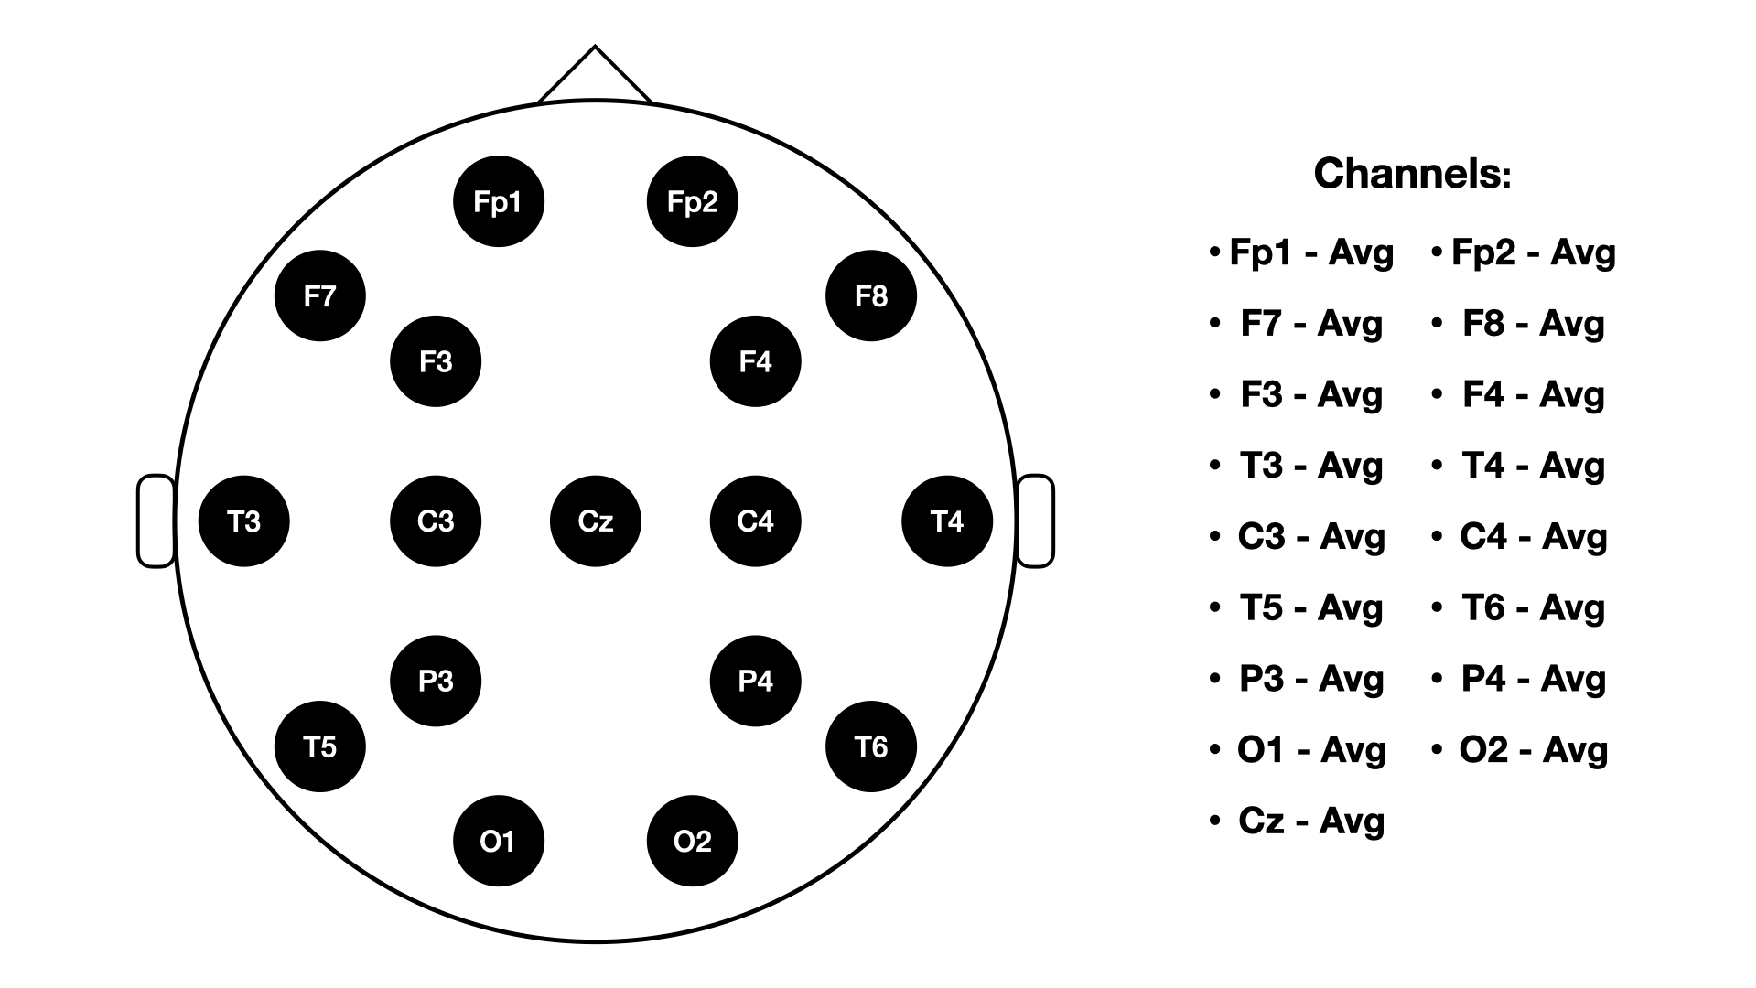
\includegraphics[width=0.8\textwidth]{images/electrodes.pdf}
    \caption{Average-referenced EEG channels across the scalp.}
    \label{fig:electrodes}
\end{figure}

\subsection{Annotation Scheme}

The annotations of the recordings were created by expert EEG annotators associated with Temple University and the Neural Engineering Data Consortium (NEDC). Each artifact event is described by a set of fields:

\textbf{channel} - The EEG channel affected by the artifact.

\textbf{start\_time} - The time, in seconds, when the artifact starts

\textbf{stop\_time} - The time, in seconds, when the artifact ends.

\textbf{label} - The type of artifact.

\textbf{confidence} - A numerical score indicating the confidence of the annotation.\\

The TUAR corpus defines a set of standard artifact classes that occur in clinical EEG recordings \cite{9353647}. Each annotated event belongs to one of the following classes:

\begin{description}

\item[\textbf{Eye movements (eyem):}] A very common artifact caused by movement of the patient’s eyes. These movements create strong signals on channels representing the frontal polar electrodes. Large spans of eye movement artifact can contribute to errors in automated seizure detection because the produced wave patterns may resemble seizure activity.

\item[\textbf{Muscle activity (musc):}] Muscle artifacts are linked to physical activity. They are quite frequent and often sudden, reflecting a state of agitation or nervousness in a patient. Their amplitude varies considerably, and their frequency is higher than 30 Hz.

\item[\textbf{Chewing (chew):}] A chewing artifact is a subset of muscle activity resulting from the tensing and relaxing of the jaw. It primarily appears on temporal channels and may show stronger activity in one hemisphere. This artifact has the characteristic high-frequency activity of muscle artifacts and commonly appears when patients move their jaw during sleep.

\item[\textbf{Shivering (shiv):}] Shivering artifact is another subset of muscle artifact that occurs when a patient shivers. It typically appears across the majority of channels. Although relatively rare, it can cause significant errors in automated analysis when present.

\item[\textbf{Electrode-related artifacts (elec):}] These artifacts are caused by issues with EEG electrodes or their connections. They include disturbances such as electrode pops, electrostatic interference, and lead artifacts, which usually appear as sudden spikes or abrupt signal changes in the affected channel.

\item[\textbf{Electrode pop (elpp):}] The electrode pop is a particular form of electrode artifact that happens as a result of a problem with a single electrode. This problem could be attributed to poor electrode attachment or air bubbles present in the conductive gel. Sometimes, the electrode pops multiple times during the recording session.

\end{description}

Segments of the EEG signal that are not annotated with any artifact label are considered \textbf{background}.

\newpage

\subsection{Dataset Analysis}

The TUAR dataset is significantly class-imbalanced, with annotation counts ranging from a few hundred to over one hundred thousand. Major classes like \texttt{musc} and \texttt{eyem} dominate, while the underrepresented minor classes contributing less than 0.1\% of the total annotations. This can result in bias toward frequent classes and weaken performance on rare artifacts. The analysis suggests the use of class weighting to compensate for the class imbalance.



\begin{figure}[H]
\centering
    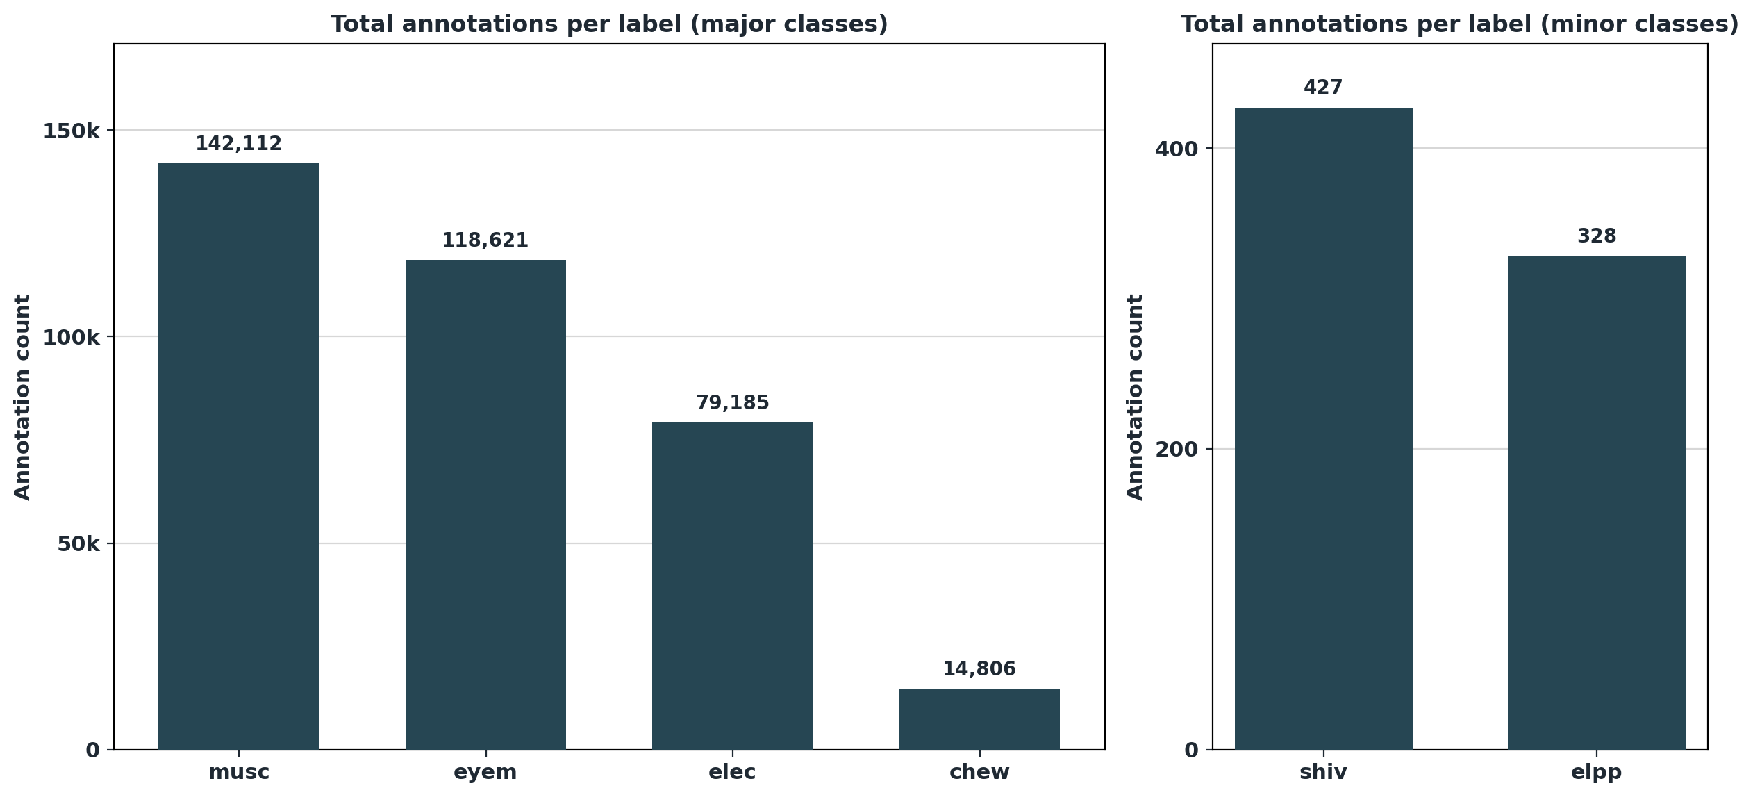
\includegraphics[width=0.9\textwidth]{images/class_annotation_counts_total.pdf}
    \caption{Total number of annotations per class in the TUAR dataset, highlighting class imbalance between major and minor categories.}
    \label{fig:annotation_counts}
\end{figure}

Balanced class distribution across splits was produced using the described dataset splitting strategy. Figure~\ref{fig:class_distribution} compares how much time each artifact class occupies in each split and in the whole dataset. It also shows that the recordings are densely annotated. 

Among the major classes, \texttt{musc} consistently represents the largest share, accounting for approximately one-fifth of the total recording time across all splits. In most classes only minor variations between splits can be observed, with the exception of \texttt{shiv}, where most of the recording containing the artifact ended up in the train split. This is due to the fact that only a small number of recordings contain \texttt{shiv}. As a result of the patient-wise splitting strategy, this distribution represents the closest achievable ratio to the target split proportions. In conclusion, the resulting distribution across splits provides a reliable basis for model evaluation.

\begin{figure}[H]
\centering
    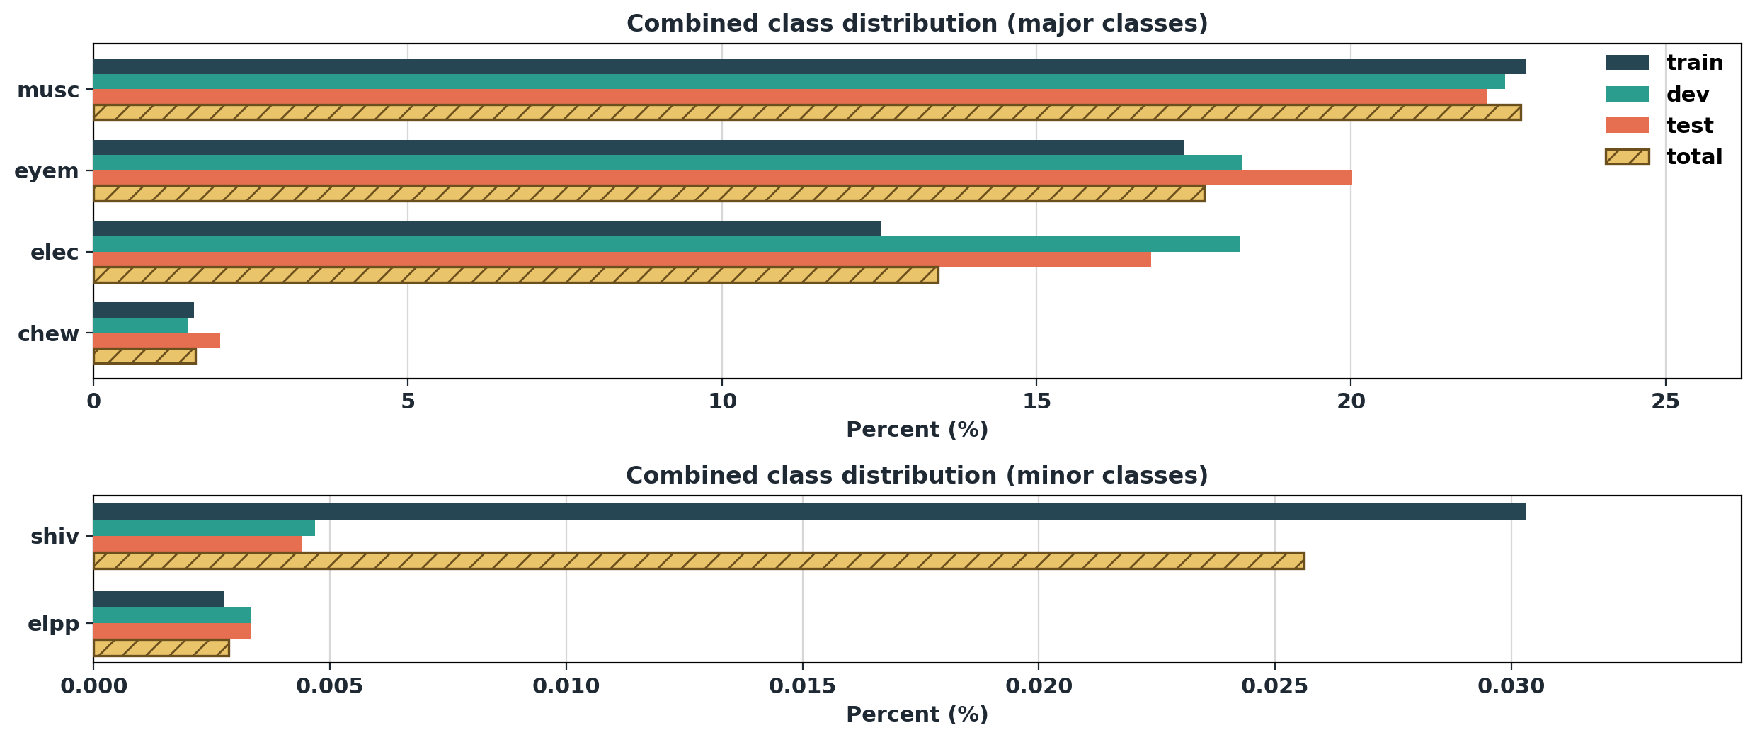
\includegraphics[width=0.9\textwidth]{images/class_distribution_pct_total_time_combined.pdf}
    \caption{Distribution of artifact classes across dataset splits based on recording time.}
    \label{fig:class_distribution}
\end{figure}

The distribution of annotation durations is shown in Figure~\ref{fig:length_distribution_3x2}. The majority of annotations are short, with most labeled segments lasting around 1 second, while some annotated sequences extend to several minutes. This highlights the uneven distribution of artifacts, where short events dominate, while longer occurrences remain relatively rare.

\begin{figure}[H]
\centering
    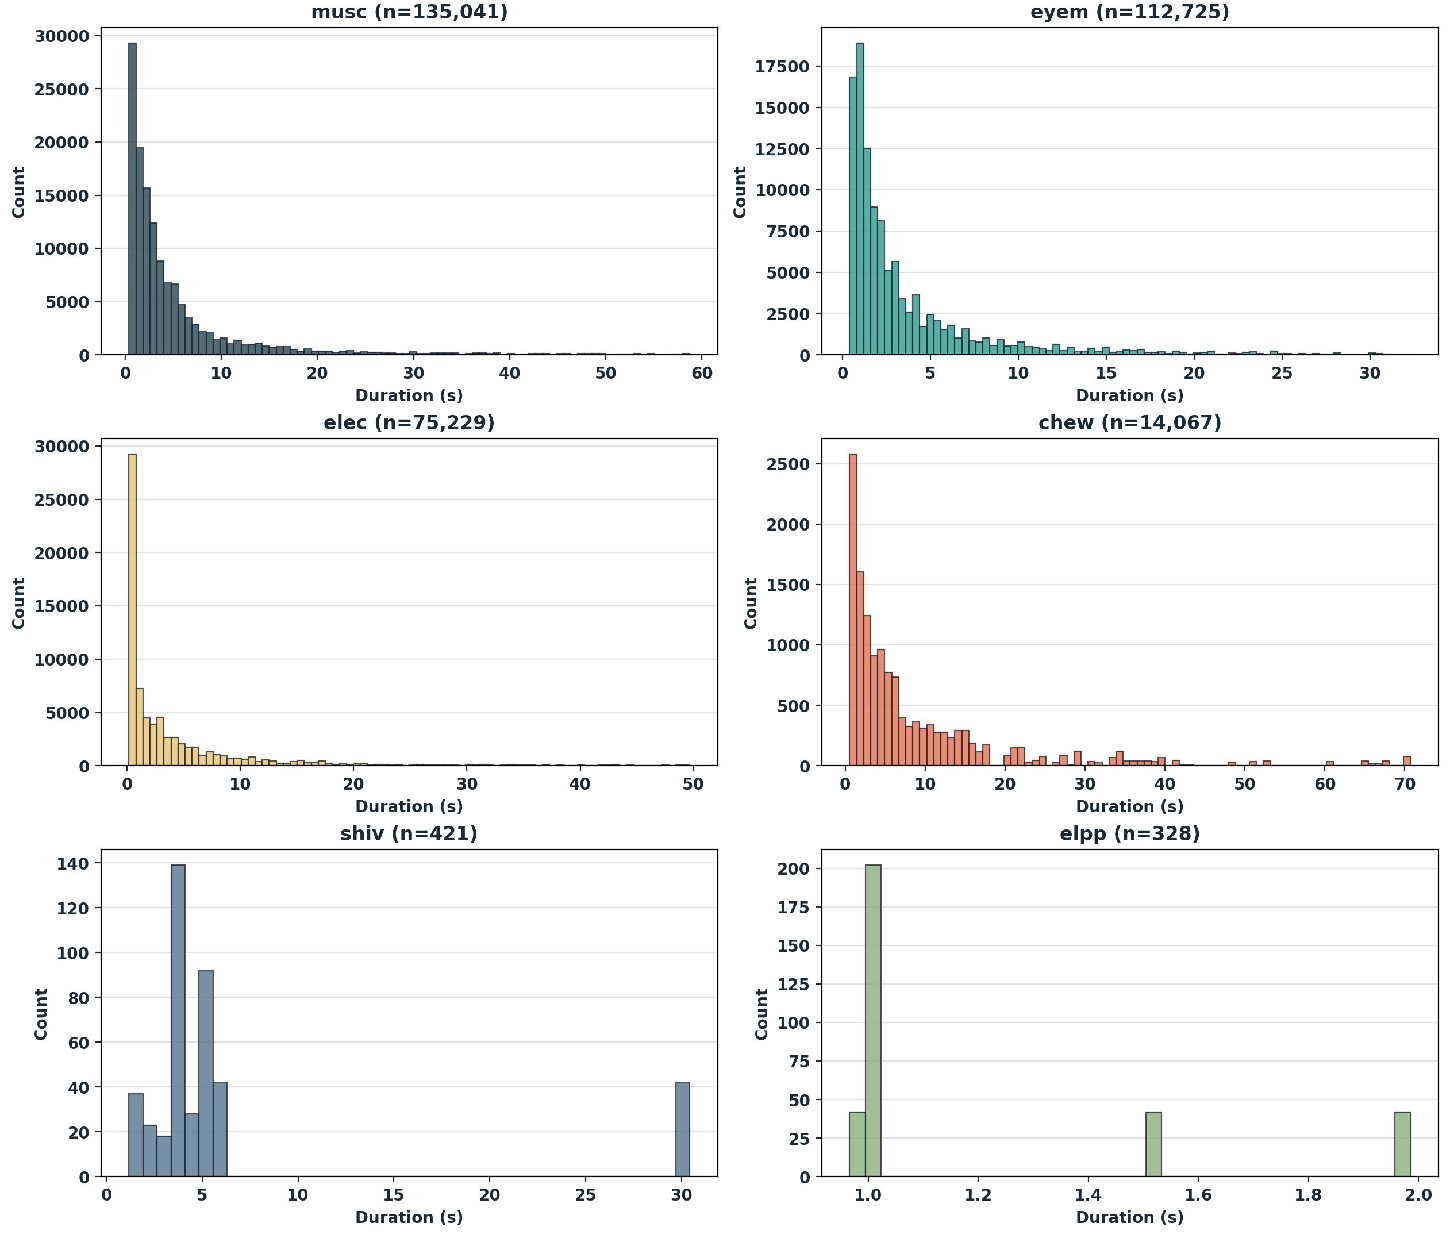
\includegraphics[width=0.9\textwidth]{images/class_annotation_length_distribution_3x2.pdf}
    \caption{Distribution of annotation durations for each artifact class. Extreme outliers are not shown for clarity.}
    \label{fig:length_distribution_3x2}
\end{figure}

The window segments of the recordings are only partially covered by annotations in most cases. This is because the majority of the artifact events are short, resulting in annotations that occupy only a fraction of a given window. However, in cases of longer artifacts, the whole segment can be covered. 

Figure~\ref{fig:eeg_window} illustrates a 4 second long window visible containing an artifact in the middle. The artifact is labeled \texttt{musc} and simultaneous present on across all channels. Outside the artifact, smoother, lower-amplitude fluctuations are present, which are characteristic of typical background EEG activity. This example illustrates how artifacts can affect multiple channels simultaneously, producing characteristic patterns in the EEG signal. 


\begin{figure}[H]
\centering
    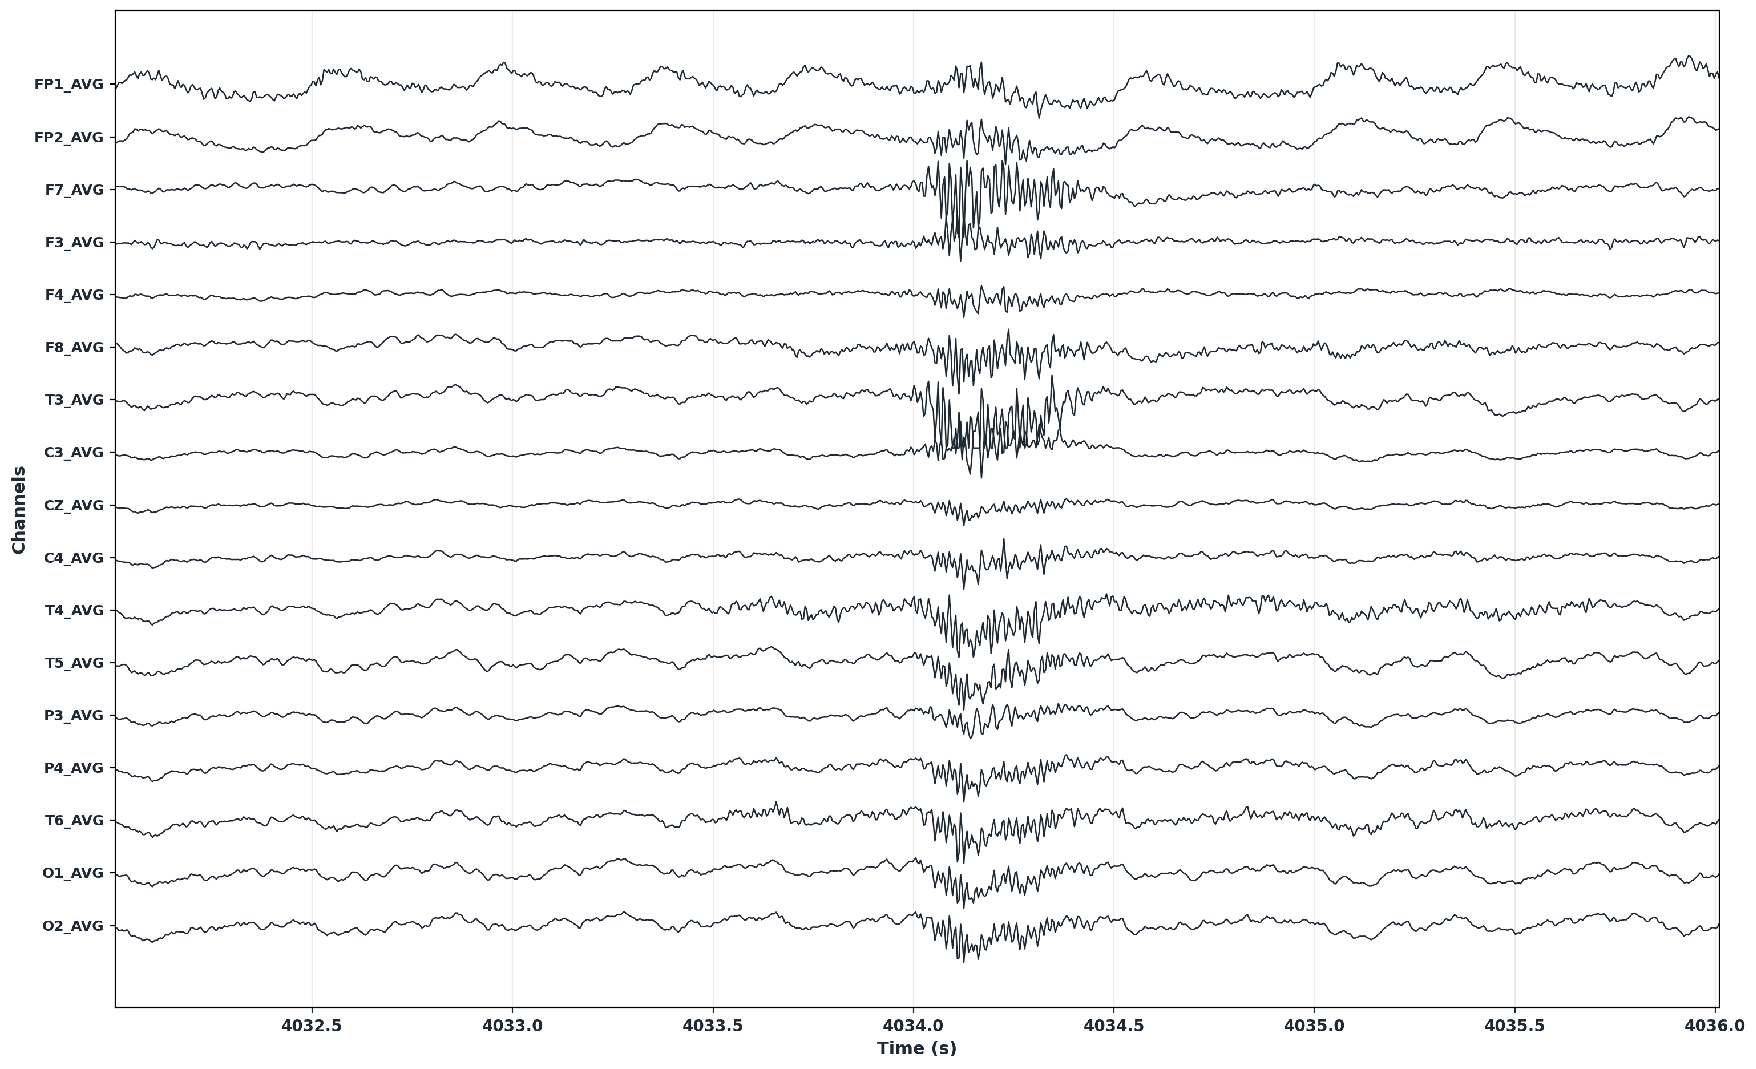
\includegraphics[width=0.9\textwidth]{images/artifact_eeg_window_4s_musc_notitle.pdf}
    \caption{Example of a 4-second EEG segment showing a \texttt{musc} artifact.}
    \label{fig:eeg_window}
\end{figure}

\section{Baseline Data Augmentation Methods}

In this section the baseline data augmentation methods are introduced. The proposed method is compared against these as described in Chapter \ref{chap:methodology} and analysed in Chapter \ref{chap:results}. The set of baseline augmentations contains six commonly used nongenerative augmentation and one WGAN-based generative method. The effects of these augmentations on classification performance are measured both separately and combined using multiple EEG classification models.

\subsection{Additive Gaussian and Pink Noise Augmentation}

Two noise-based data augmentation methods were selected: Gaussian (white) noise augmentation and pink noise augmentation, both widely used in EEG signal classification. The goal of these augmentations is to add controlled stochastic variations to the signal while preserving its structure. This reduces sensitivity to noise and reduces overfitting to the training data.

During both gaussian and pink noise augmentation, $\mathrm{RMS}_{\text{signal}}$ is computed per channel for each window $x \in \mathbb{R}^{C \times T}$, where $C$ and $T$ denote the number of EEG channels and the number of time samples in the window.

\[
\mathrm{RMS}_{\text{signal}} = \sqrt{\frac{1}{T} \sum_{t=1}^{T} x_t^2}
\]

The signal-to-noise ratio (SNR) defined in decibels is converted into a linear ratio and then used to calculate the target amplitude of the noise relative to the original signal.

\[
\mathrm{SNR}_{\text{linear}} = 10^{\mathrm{SNR}_{\text{dB}} / 20}
\]

\[
\mathrm{RMS}_{\text{noise}} = \frac{\mathrm{RMS}_{\text{signal}}}{\mathrm{SNR}_{\text{linear}}}
\]


The Gaussian augmentation assembles the noise signal by generating samples from a standard normal distribution. It is then scaled accordingly using the signal-to-noise ratio and the scaled noise is added to the original EEG signal.

Instead of generating noise directly in the time domain, the pink noise augmentation uses a frequency-domain representation. First, a random spectrum is created and then reshaped to follow a distribution $1/f$ by scaling each frequency component inversely with the square root of its frequency. The spectrum is transformed back to the time domain with the inverse Fourier transform that results in a temporally correlated noise signal. The signal is normalised, scaled using the signal-to-noise ratio, and added to the original signal similar to the gaussian augmentation.

\[
\setlength{\arraycolsep}{40pt}
\begin{array}{cc}
\textbf{Gaussian Noise} & \textbf{Pink Noise} \\[10pt]

n_t \sim \mathcal{N}(0,1) 
&
S(f) \sim \mathcal{N}(0,1)
\\[10pt]

n_t' = n_t \cdot \mathrm{RMS}_{\text{noise}}
&
S(f) \leftarrow \frac{S(f)}{\sqrt{f}}
\\[10pt]

\tilde{x}_t = x_t + n_t'
&
p_t = \mathcal{F}^{-1}(S(f))
\\[10pt]

&
p_t' = \frac{p_t}{\mathrm{RMS}(p)} \cdot \mathrm{RMS}_{\text{noise}}
\\[10pt]

&
\tilde{x}_t = x_t + p_t'

\end{array}
\]

Both methods follow the same scaling strategy, the difference is the structure of the generated noise. Gaussian noise introduces unstructured perturbations, improving general robustness, while pink noise generates temporally correlated signals that better reflect EEG characteristics, resulting in a more physiologically realistic augmentation. 

\subsection{Channel Dropout}

Channel dropout is a basic augmentation technique with two main advantages: it improves model generalisation and simulates the temporary loss or corruption of an electrode. During clinical EEG recording, hardware issues and patient movements can result in the loss of channels. This augmentation forces the model to learn to handle these situations by randomly removing information from selected channels during training.

Channel dropout selects a subset of the channels randomly and sets their entire time series to zero. The augmented signal $\tilde{x}_c$ is defined as:

\[
\tilde{x}_c =
\begin{cases}
0, & \text{if } c \in \mathcal{D} \\
x_c, & \text{otherwise}
\end{cases}
\]

where $\mathcal{D} \subset \{1, \dots, C\}$ represents the set of dropped channels. 

The augmentation is controlled by two parameters, the probability of its application and the number of channels dropped determined by a predefined fraction parameter. 

Dropping channels is a stronger regularisation techniques than noise-based augmentations, but if applied too aggressively, it can negatively affect performance due to
information loss.

\subsection{Temporal Augmentations}

Temporal augmentations are time domain transformations of the data that modify the temporal structure of EEG signals, but preserve their physiological characteristics. Without augmentations affecting the time domain, the model may learn positional biases due to fixed window size and stride. This method helps the model avoid overfitting and also gives the dataset increased variability by using a combined time domain augmentation strategy, consisting of random cropping followed by temporal shifting.

Random subsegment of the original signal is cropped with length $T' = \alpha T$, where $\alpha \in (0, 1]$ is the crop fraction. If the crop starts at index $s$, the cropped signal is:

\[
x_{\text{crop}} = x[:,\, s : s + T']
\]

Then zero padding is added to the cropped segment to reconstruct the original window length $T$:

\[
x_{\text{pad}} = \text{pad}(x_{\text{crop}})
\]

Following the cropping, temporal shifting is applied to the padded signal. A shift value $\Delta \in [-\delta T, \delta T]$ is sampled, where $\delta \in [0,1]$ controls the maximum shift fraction. The signal is shifted either left or right, and missing values are filled with zeros, randomizing the patter positions within the window: 

\[
\tilde{x}(t) =
\begin{cases}
0, & t < \Delta \ \text{or} \ t \geq T + \Delta \\
x_{\text{pad}}(t - \Delta), & \text{otherwise}
\end{cases}
\]

This augmentation is a transformation pipeline with the goal to simulate realistic variability in artifact positioning by removing a portion of the signal and then randomly shifting the remaining content within the window. This is beneficial in most EEG classification settings, where artifacts can occur anywhere within the window, including at the edges.

\subsection{Segment Recombination}

Segment recombination is a time domain augmentation technique similar to temporal augmentations, with the difference that instead of applying local transformations like shifting or cropping, it restructures the signal by rearranging its internal segments.

The first step is to divide the signal into $K$ non-overlapping segments and rearrange them using a random permutation $\pi$: 

\[
x = \left[ x^{(1)}, x^{(2)}, \dots, x^{(K)} \right]
\]

\[
\tilde{x} = \left[ x^{(\pi(1))}, x^{(\pi(2))}, \dots, x^{(\pi(K))} \right]
\]

Local patterns within each segment are preserved but their original temporal ordering is disrupted. 

The problem with the concatenation is that the assembled signal is discontinuous, unrealistic high-frequency artifacts. For reducing this effect, a phase-based correction is used, in which the Fourier transform of the shuffled signal $\tilde{x}_c(t)$ is computed for each channel:

\[
X_c(f) = \mathcal{F}\{\tilde{x}_c(t)\}
\]

The signal can be represented in terms of its magnitude and phase in the following form:

\[
X_c(f) = \lvert X_c(f) \rvert \cdot e^{i \phi_c(f)}
\]

where $\phi_c(f)$ denotes the phase. 
Discontinuities in the time domain are represented by large phase inconsistencies, that are smoothed here producing the corrected phase $\phi_c^{\text{corr}}(f)$. The signal is then reconstructed using the inverse Fourier transform:

\[
\hat{x}_c(t) = \mathcal{F}^{-1} \left( |X_c(f)| \cdot e^{i \phi_c^{\text{corr}}(f)} \right)
\]

This segment recombination augmentation can produce high temporal variability while keeping the local characteristics of the signal largely preserved. This helps the model become less sensitive to exact timing and focus more on the underlying patterns in the signal.

\subsection{Mixup-like Window Blending}

This augmentation technique applies a window level Mixup strategy. In classical Mixup, both inputs and labels are interpolated, but a common alternative is to preserve the original target label and introduce small, controlled perturbations using additional EEG windows.

For a given target window $x_{\text{target}}$, two auxiliary windows $x_{\text{noise1}}$ and $x_{\text{noise2}}$ are randomly sampled from the dataset. Then these auxiliary signals are averaged using random weights $w_1$, $w_2$, where $w_1 + w_2 = 1$.

\[
x_{\text{noise}} = w_1 x_{\text{noise1}} + w_2 x_{\text{noise2}}
\]

The final augmented signal is then computed as a weighted combination of the target window and the generated noise signal: 

\[
x_{\text{aug}} = 0.9 \, x_{\text{target}} + 0.1 \, x_{\text{noise}}
\]

The original target label is assigned to the augmented window, since the target signal contributes most to the resulting signal, while the auxiliary signals are only used to introduce minor perturbations. 

In contrast to gaussian or pink noise augmentation that uses fully synthetic noise, this method introduces variability using actual EEG recordings. The result is a biologically more realistic signal and may better support generalisation to real-world data.

\subsection{GAN-Based Synthetic Data Generation}

A common method for improving the variability of the dataset is synthetic data generation using generative models. Generative Adversarial Networks (GANs) have been used to extend a base dataset, with the architecture consisting of a Generator that learns to transform input noise into synthetic data, and a Discriminator that learns to distinguish between generated and real ones. 

For the implemented data augmentation, a network based on Wasserstein Generative Adversarial Network with Gradient Penalty (WGAN-GP) \cite{gulrajani2017} was trained for generating synthetic data for each class in the dataset. The WGAN-GP architecture consists of a generator–critic pair trained using the Wasserstein GAN framework with additional gradient penalty. 

The generator $G$ is designed to map a latent vector $z \in \mathbb{R}^{d}$, that is sampled from a standard normal distribution $z \sim \mathcal{N}(0, I)$, to a synthetic EEG window $\hat{x} \in \mathbb{R}^{C \times T}$. At first, $z$ is projected into a feature space, from where it is refined through a sequence of upsampling blocks consisting of linear interpolation, convolution, normalisation, and an activation function. After the finale block the feature tensor is converted into EEG channels using a final convolution layer. It is then resized and passed through a hyperbolic tangent activation to produce the final synthetic window. 

The critic $C$ acts as the discriminator in a classical GAN architecture, but instead of returning a probability, it estimates the Wasserstein distance between real and generated data distributions. The convolutional backbone uses progressive temporal downsampling while it captures local and global dependencies in signal. After the backbone an average pooling operation is applied and the final critic score is computed using linear projection. 

The objective of the WGAN-GP framework is to approximate the Wasserstein-1 distance between the real data distribution $p_r$ and the distribution $p_g$ generated by the model. For this the following critic loss is used:

\[
\mathcal{L}_C = \mathbb{E}_{x \sim p_g}[C(x)] - \mathbb{E}_{x \sim p_r}[C(x)] + \lambda \mathcal{L}_{\mathrm{GP}}
\]

where $\lambda$ is a regularisation coefficient and $\mathcal{L}_{\mathrm{GP}}$ is the gradient penalty term.

The gradient penalty is computed on interpolated samples:

\[
\hat{x} = \epsilon x_r + (1 - \epsilon)x_g, \quad \epsilon \sim \mathcal{U}(0,1),
\]
\[
\mathcal{L}_{\mathrm{GP}} = \mathbb{E}_{\hat{x}} \left[ \left( \left\| \nabla_{\hat{x}} C(\hat{x}) \right\|_2 - 1 \right)^2 \right].
\]

Wasserstein distance requires the 1-Lipschitz constraint and this penalty enforces it by keeping the gradients of the critic around 1.

The generator loss function used is the following:

\[
\mathcal{L}_G = -\mathbb{E}_{z \sim p(z)} \left[ C(G(z)) \right]
\]

This model is designed to be trained separately for each EEG class, and saved as independent, specialised models for synthetic data generation. Adding generated EEG window to a real dataset can improve class balance and enhance model generalisation.

\newpage

\section{Models for EEG Classification}

This chapter introduces the selected models used for evaluation of the proposed and baseline augmentations. The selection contains different structural properties and includes both simpler and more advanced models, with the goal of assessing how the augmentation techniques influence different types of model architectures. 

\subsection{EEGNet}

EEGNet \cite{Lawhern_2018} is a widely used, compact convolutional network that has become a standard baseline model in many EEG-related studies. The main advantage of the model is that it uses a small number of parameters while still capturing the temporal and spatial characteristics of EEG signals, mirroring classical EEG processing pipelines. 

First, it learns temporal patterns such as short-term waveform changes, local signal dynamics, and oscillatory patterns from the signal over time by using temporal convolution with kernel moving along the time axis. Then a spatial depthwise convolution is applied using kernel operating across the entire channel dimension but not along the time axis. The role of this layer is to learn how information from the EEG channels should be combined. A depthwise temporal convolution processes each feature map along time refining temporal information within each learned channel-specific representation, followed by a pointwise convolution step combining these depthwise outputs across channels. Finally, the features are pooled and passed to a linear layer to obtain the class logits.

\begin{figure}[H]
\centering
    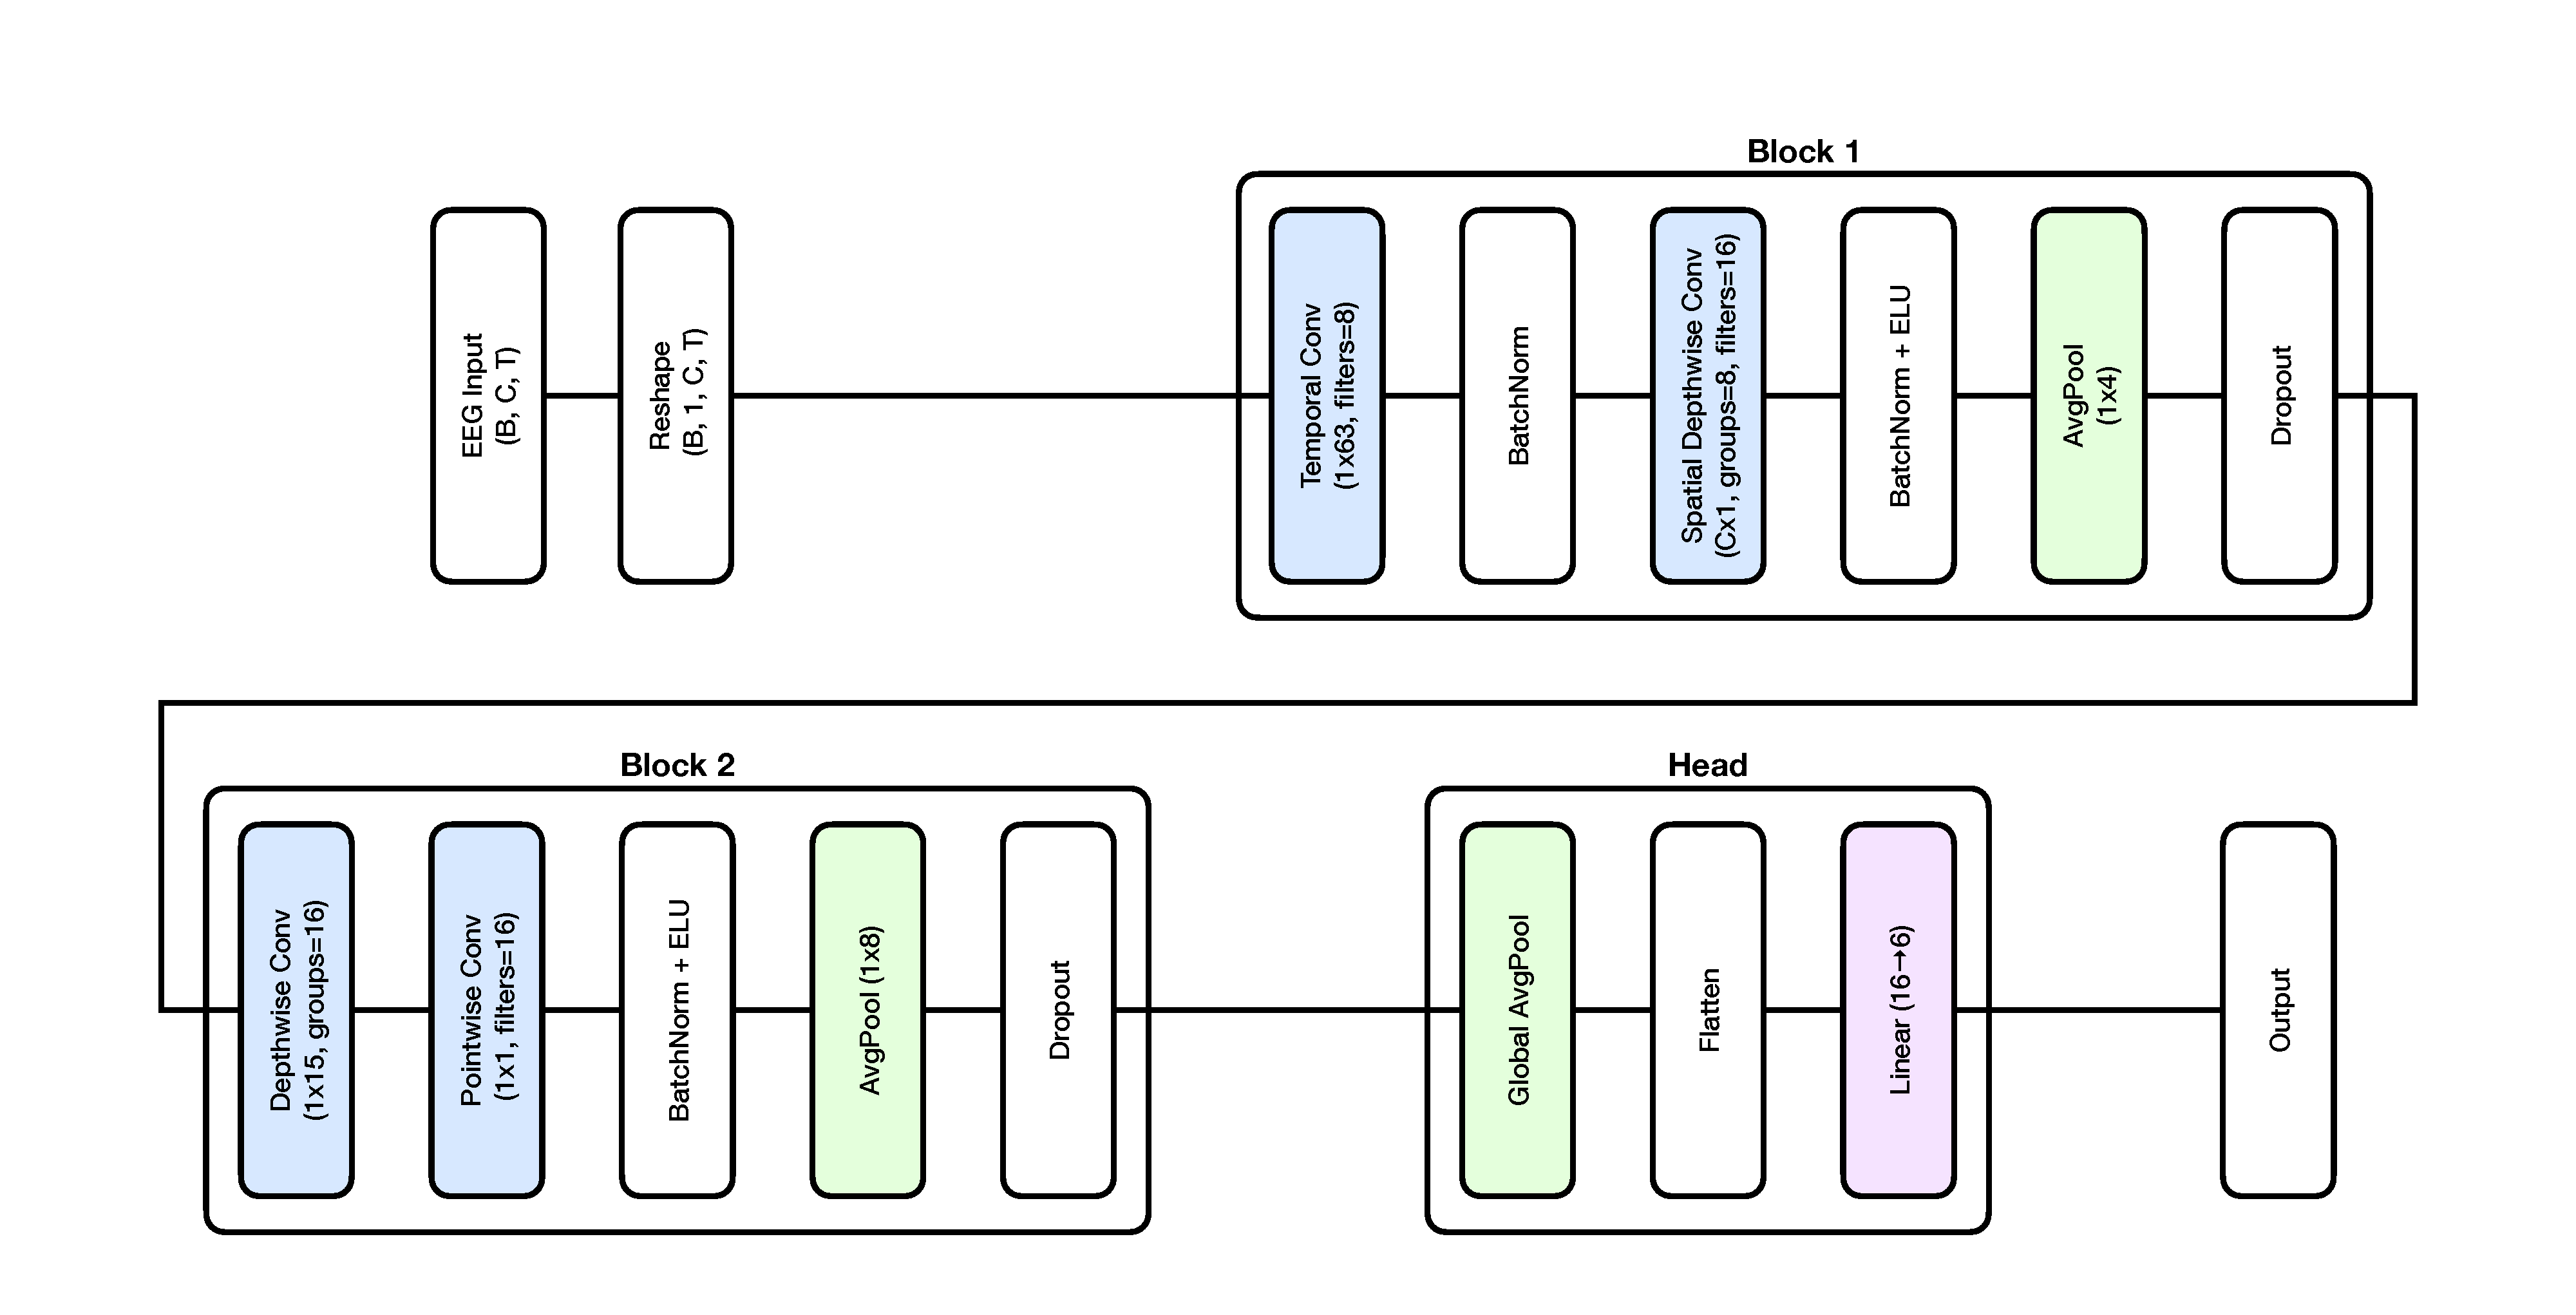
\includegraphics[width=0.9\textwidth]{images/EEGNet.pdf}
    \caption{EEGNet model structure showing Block 1 (temporal extraction and spatial filtering), Block 2 (depthwise temporal refinement), and Head (classification output).}
    \label{fig:EEGNet}
\end{figure}

\subsection{EEGNeX}

EEGNeX \cite{CHEN2024105475} keeps the same goal of learning temporal and spatial structure of the signal as the EEGNet, but it introduces a deeper and more flexible convolutional architecture. EEGNeX is a five-block, convolution only design with two temporal convolution layers, a depthwise spatial convolution across all channels, and two temporal convolutions with dilation. This design makes it capable of capturing long-range temporal dependencies more effectively than its predecessor.

Using multiple temporal convolution layers, the model is able to learn more complex patterns compared to EEGNet which uses only one at the beginning. Another important difference is dilation. Dilated temporal refinement increases the spacing between kernel elements during convolution. The result is a larger temporal context window without an increased kernel size or number of parameters. Batch normalisation is applied after each convolution layer to maintain stable training and dropout is applied after pooling to avoid overfitting.

EEGNeX is a newer architecture that is not as widely adopted as EEGNet, but it has demonstrated competitive performance among CNN-based models for EEG classification tasks.

\begin{figure}[H]
\centering    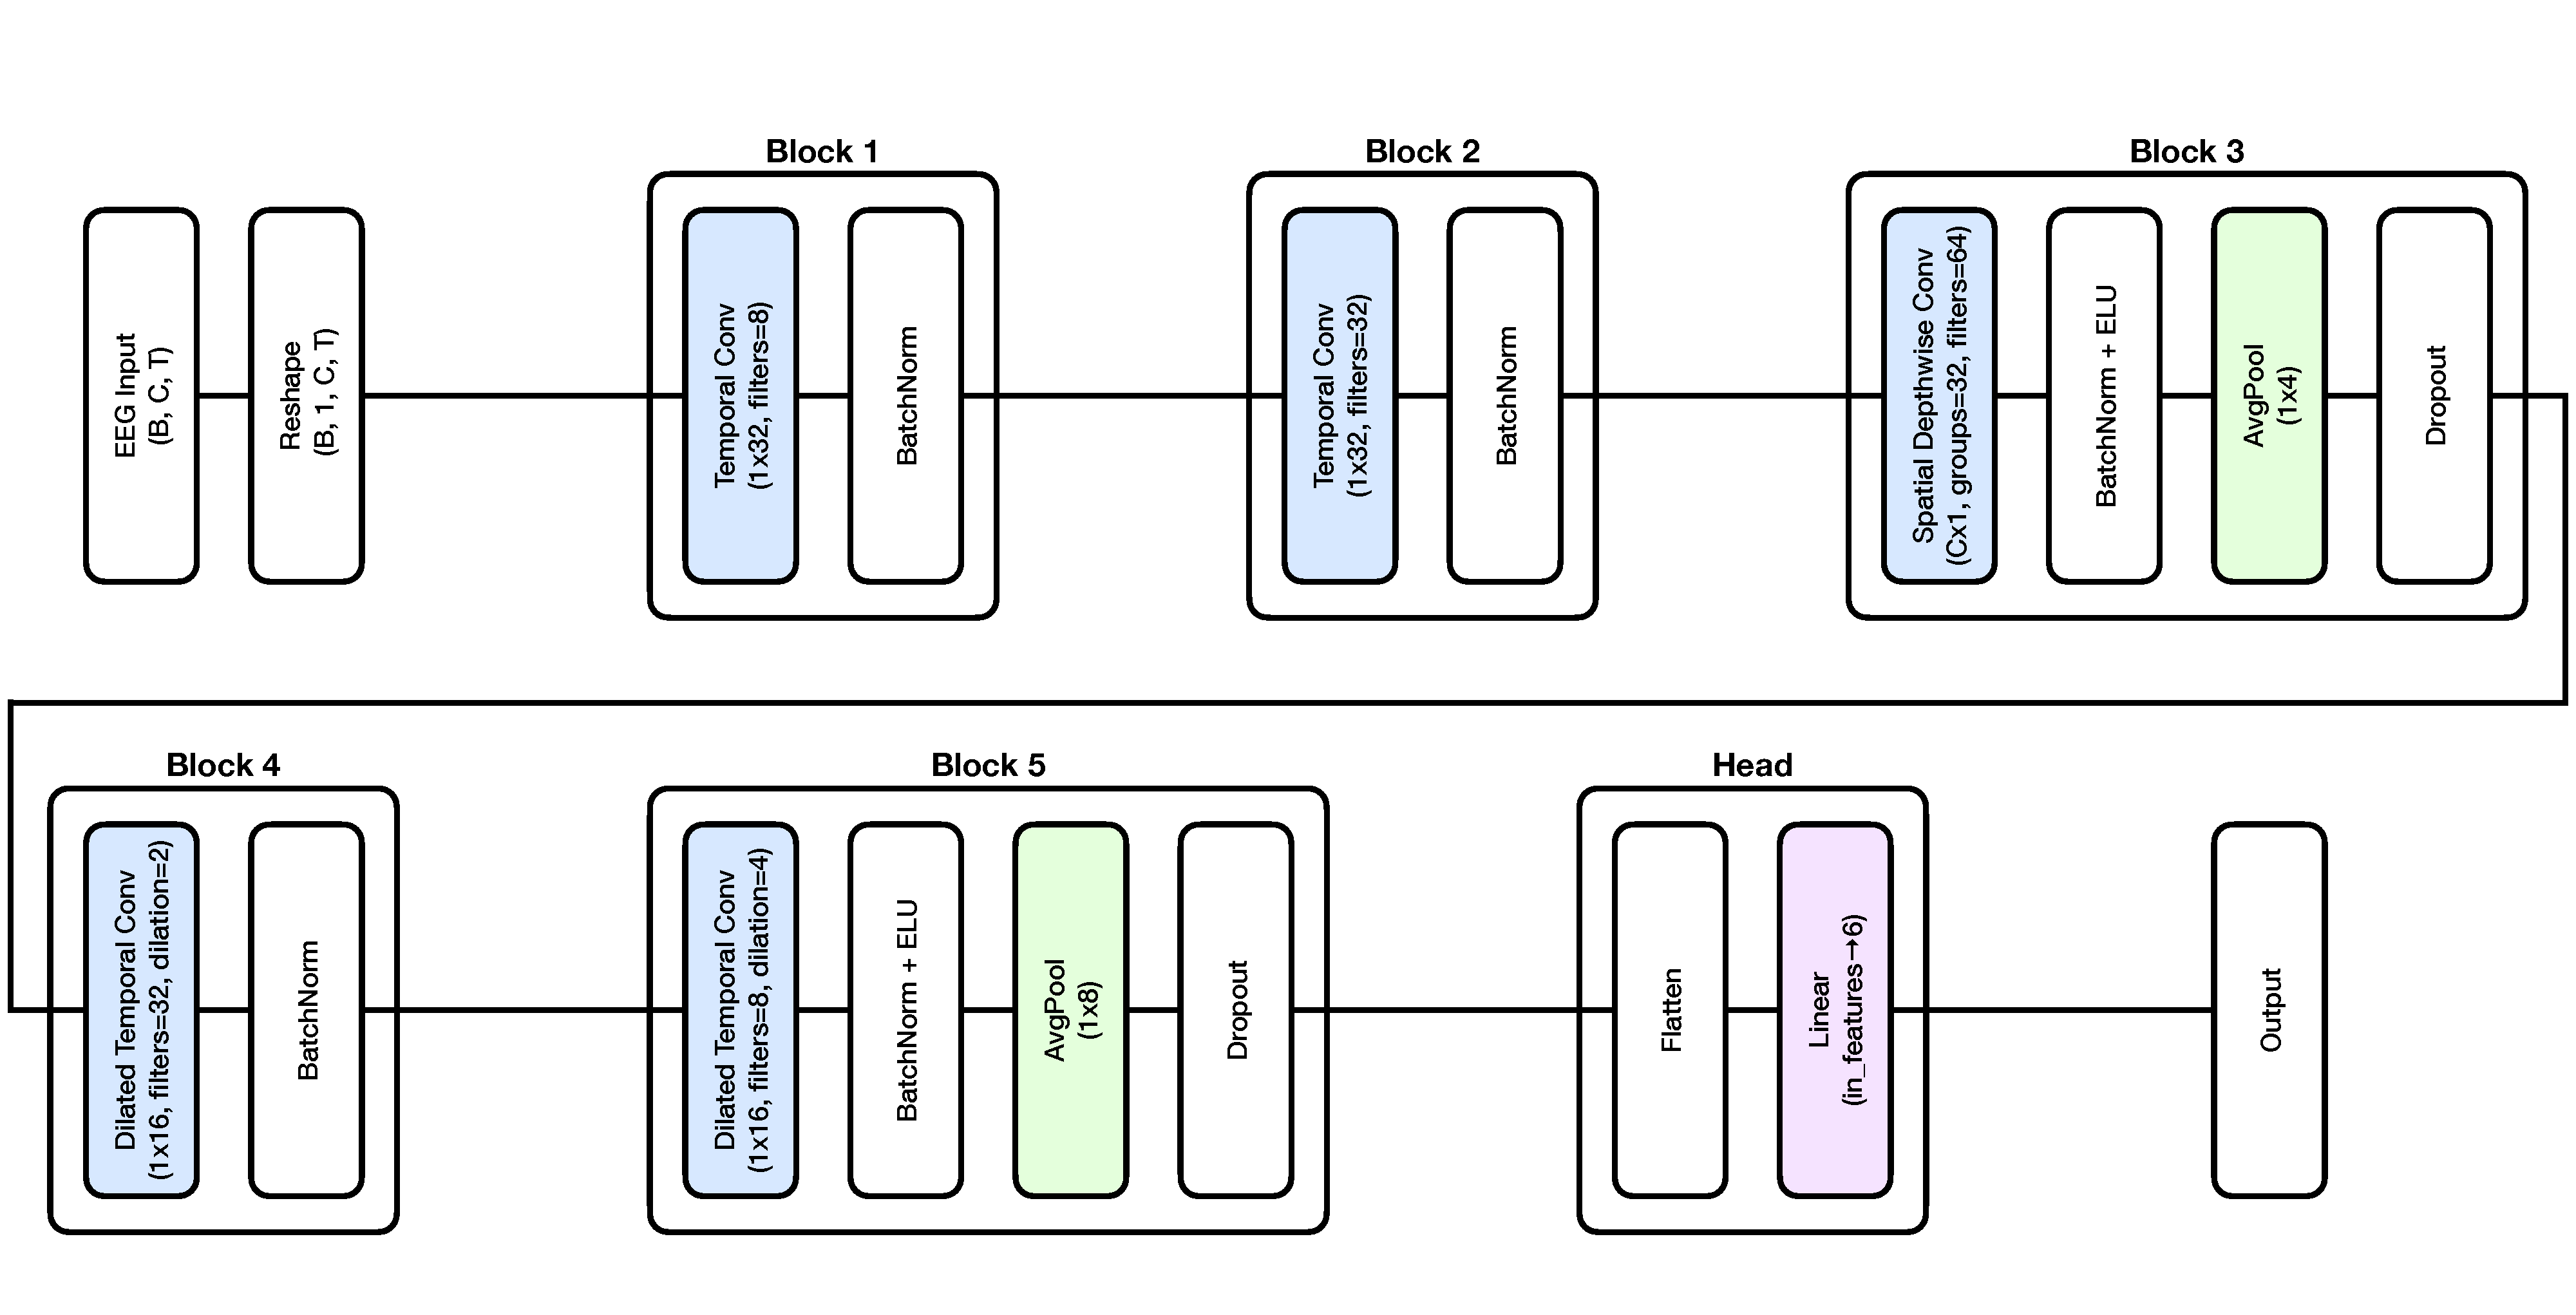
\includegraphics[width=1\textwidth]{images/EEGNeX.pdf}
    \caption{EEGNeX model structure showing Blocks 1-2 (temporal extraction), Block 3 (spatial convolution), Blocks 4-5 (dilated refinement), and Head (classification output).}
    \label{fig:EEGNeX}
\end{figure}

\newpage

\subsection{EEGInceptionERP}

The EEGInceptionERP \cite{EEGInceptionERP} is one of the strongest CNN-based architectures. It extends earlier models by introducing a design that enables multi-scale temporal feature extraction, but remains lightweight compared to other baseline EEG classification models.

The first block contains multi-scale temporal feature extraction and spatial filtering, which are computed on three parallel branches using different kernel sizes. This allows the model to capture both long-term dependencies and short events. The second block refines the extracted features using a similar parallel temporal convolution with smaller kernel sizes, where the goal is to learn finer temporal details of the signal. The third block of the model implements the refinement stage, where convolutions are applied for the extracted feature maps of the previous block followed by the classification head, which produces the output logits corresponding to the target classes.

These components form an efficient and expressive architecture that extends the capabilities of EEGNet and remains more lightweight than EEGNeX.

\begin{figure}[H]
\centering
    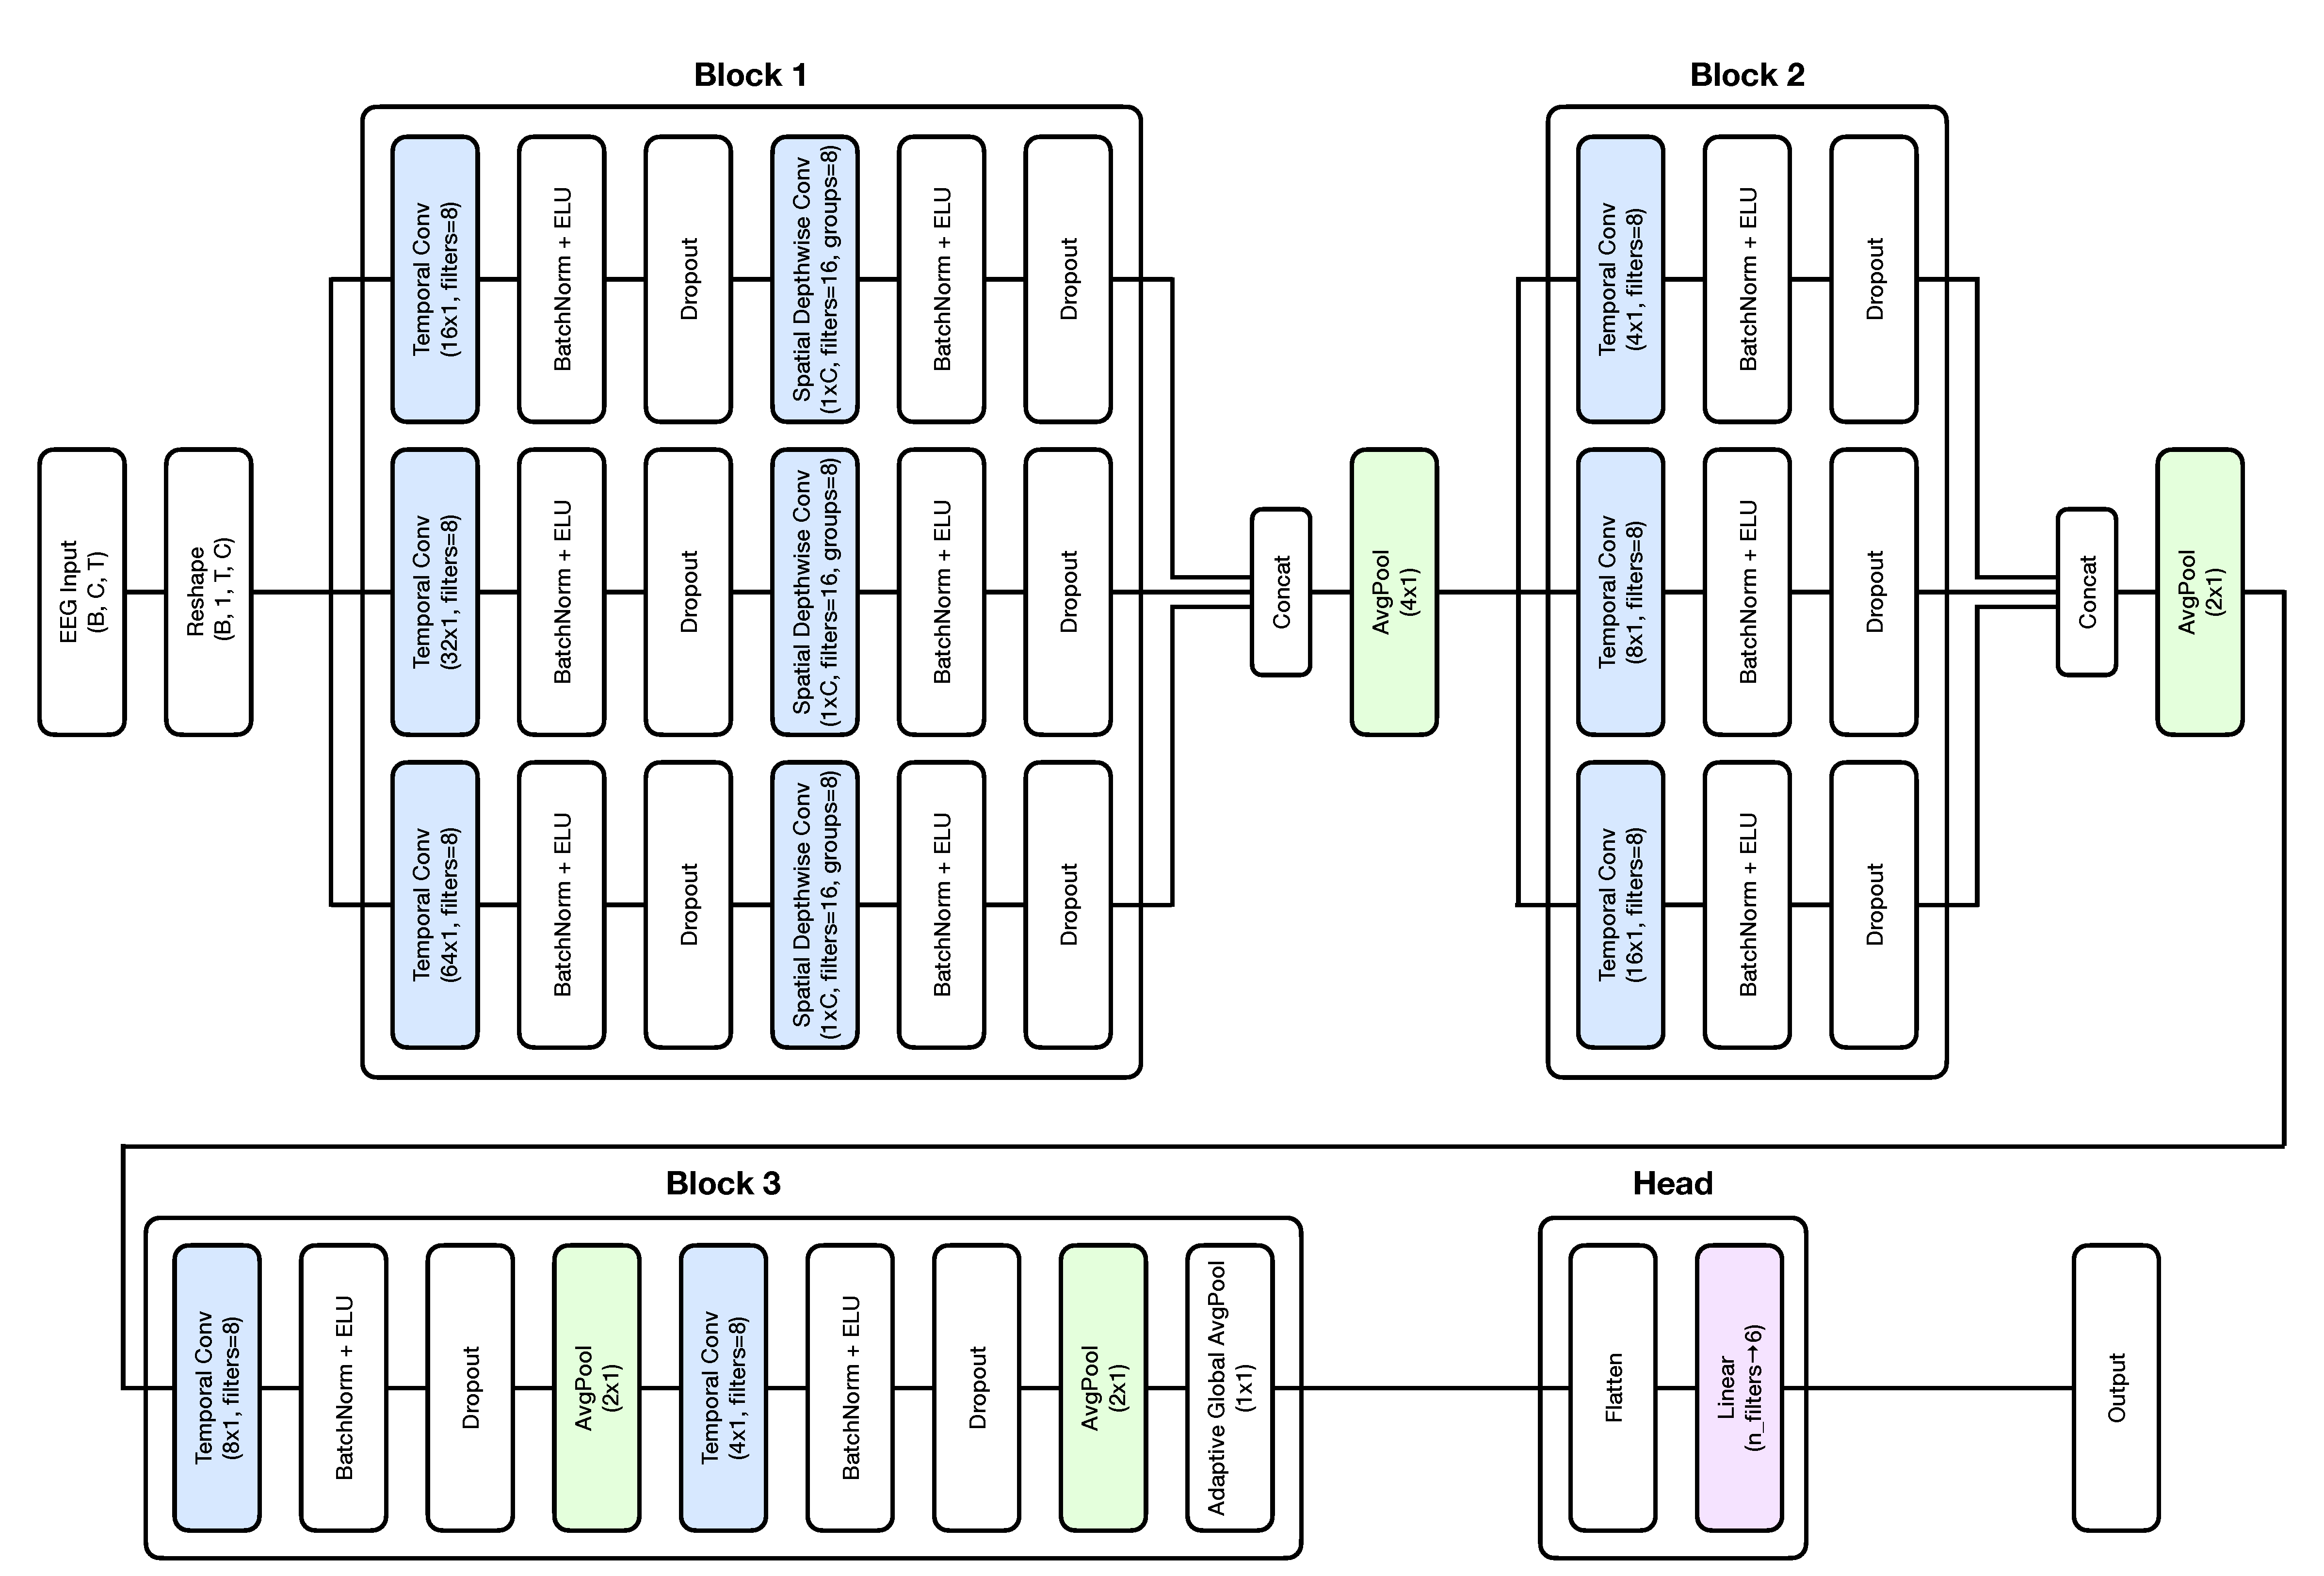
\includegraphics[width=1\textwidth]{images/EEGInceptionERP.pdf}
    \caption{EEGInceptionERP model structure showing Block 1 (multi-scale temporal and spatial extraction), Block 2 (multi-scale temporal refinement), Block 3 (refinement stage), and Head (classification output).}
    \label{fig:EEGInceptionERP}
\end{figure}

\subsection{CNN-LSTM}

This is a CNN-LSTM \cite{inproceedings} hybrid model because it combines convolutional feature extraction with sequence learning methods. It is important to include baseline CNN-RNN models in the experimentation as they serve as an intermediate step between CNN models and more advanced state-of-the-art solutions.

The architecture can be divided into three blocks. The first two blocks contain a 1D convolutional feature extractor similar to EEGNet and EEGNeX, where the EEG channels are treated as input channels of the convolution, and the kernels move only along the time axis. After the two stage CNN part the sequence is passed to the LSTM block that models temporal dependencies in the extracted features, allowing the model to learn contextual information across the entire EEG window segment. In this implementation a bidirectional, multi-layer LSTM is used to allow deeper understanding by processing the sequence in both forward and backward directions. The outputs of the forward and backward passes are combined and the last timestep of the LSTM is selected as the final sequence representation used for classification. This representation is further passed on to the classifier, where the output from the fully connected layer produces logits.

CNN–LSTM architectures have been shown to provide strong performance in EEG classification tasks, outperforming earlier convolutional models while remaining less complex than more advanced approaches. They are also commonly used in practice for time-series and biomedical signal processing tasks due to this balance. For these reasons, this architecture was chosen for the experiments.

\begin{figure}[H]
\centering
    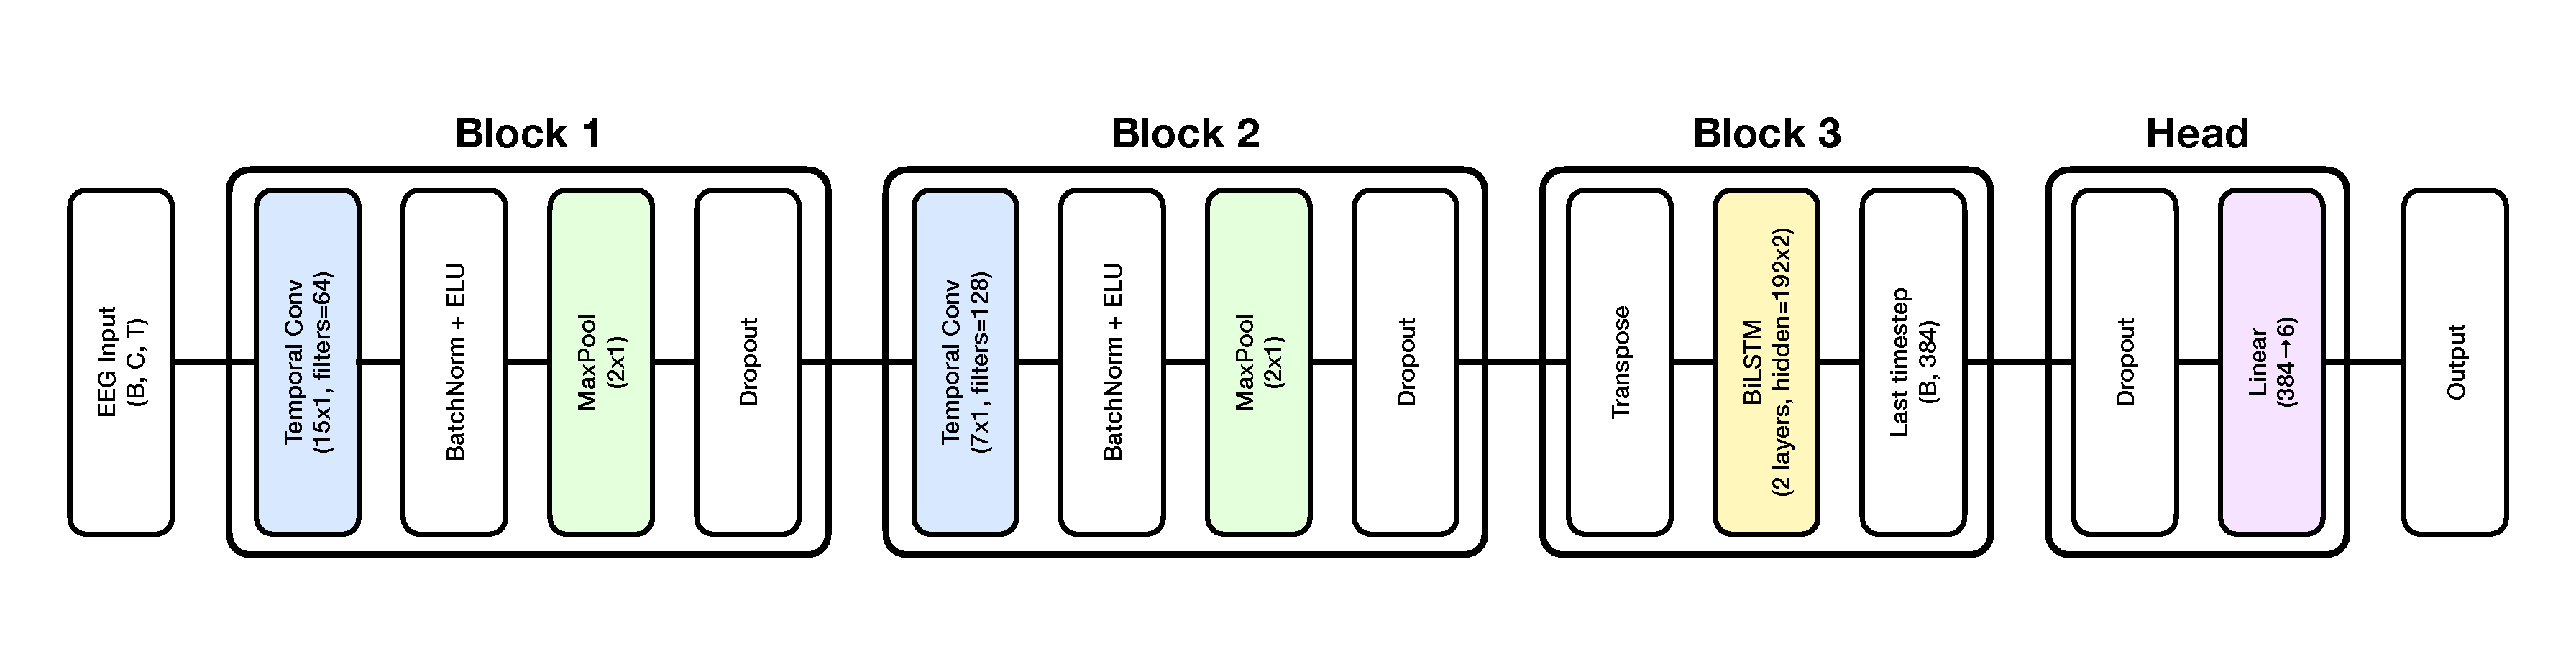
\includegraphics[width=1\textwidth]{images/CNNLSTM.pdf}
    \caption{CNN–LSTM model structure showing Blocks 1–2 (temporal convolutional extraction), Block 3 (bidirectional LSTM sequence modeling), and Head (classification output).}
    \label{fig:CNN-LSTM}
\end{figure}

\subsection{EEGConformer}

EEG-Conformer \cite{Conformer} is a convolution-first model augmented with a lightweight transformer encoder. This hybrid model demonstrated top performance in many EEG signal classification tasks.

The input sequence first passes through the shallow convolutional patch embedding block. A temporal convolution layer captures local temporal patterns along the time axis and a spatial convolution explores relationships between different channels. The second block contains the transformer encoder, where several stacked blocks of multihead attention mechanism and a feed-forward network with skip connections refine the token representations of the signal step by step. This allows the model to capture longer dependencies and global contextual information that cannot be effectively modeled by convolutional operations alone. EEGConformer uses pre-layer normalisation, which means that layer normalisation is applied before the self-attention and feed-forward sublayers as in most modern Transformer designs. The output sequence of the encoder is flattened and passed to final classification head.

This model was included in the set of selected models because of its state-of-the-art performance on many benchmark EEG classification tasks.

\begin{figure}[H]
\centering
    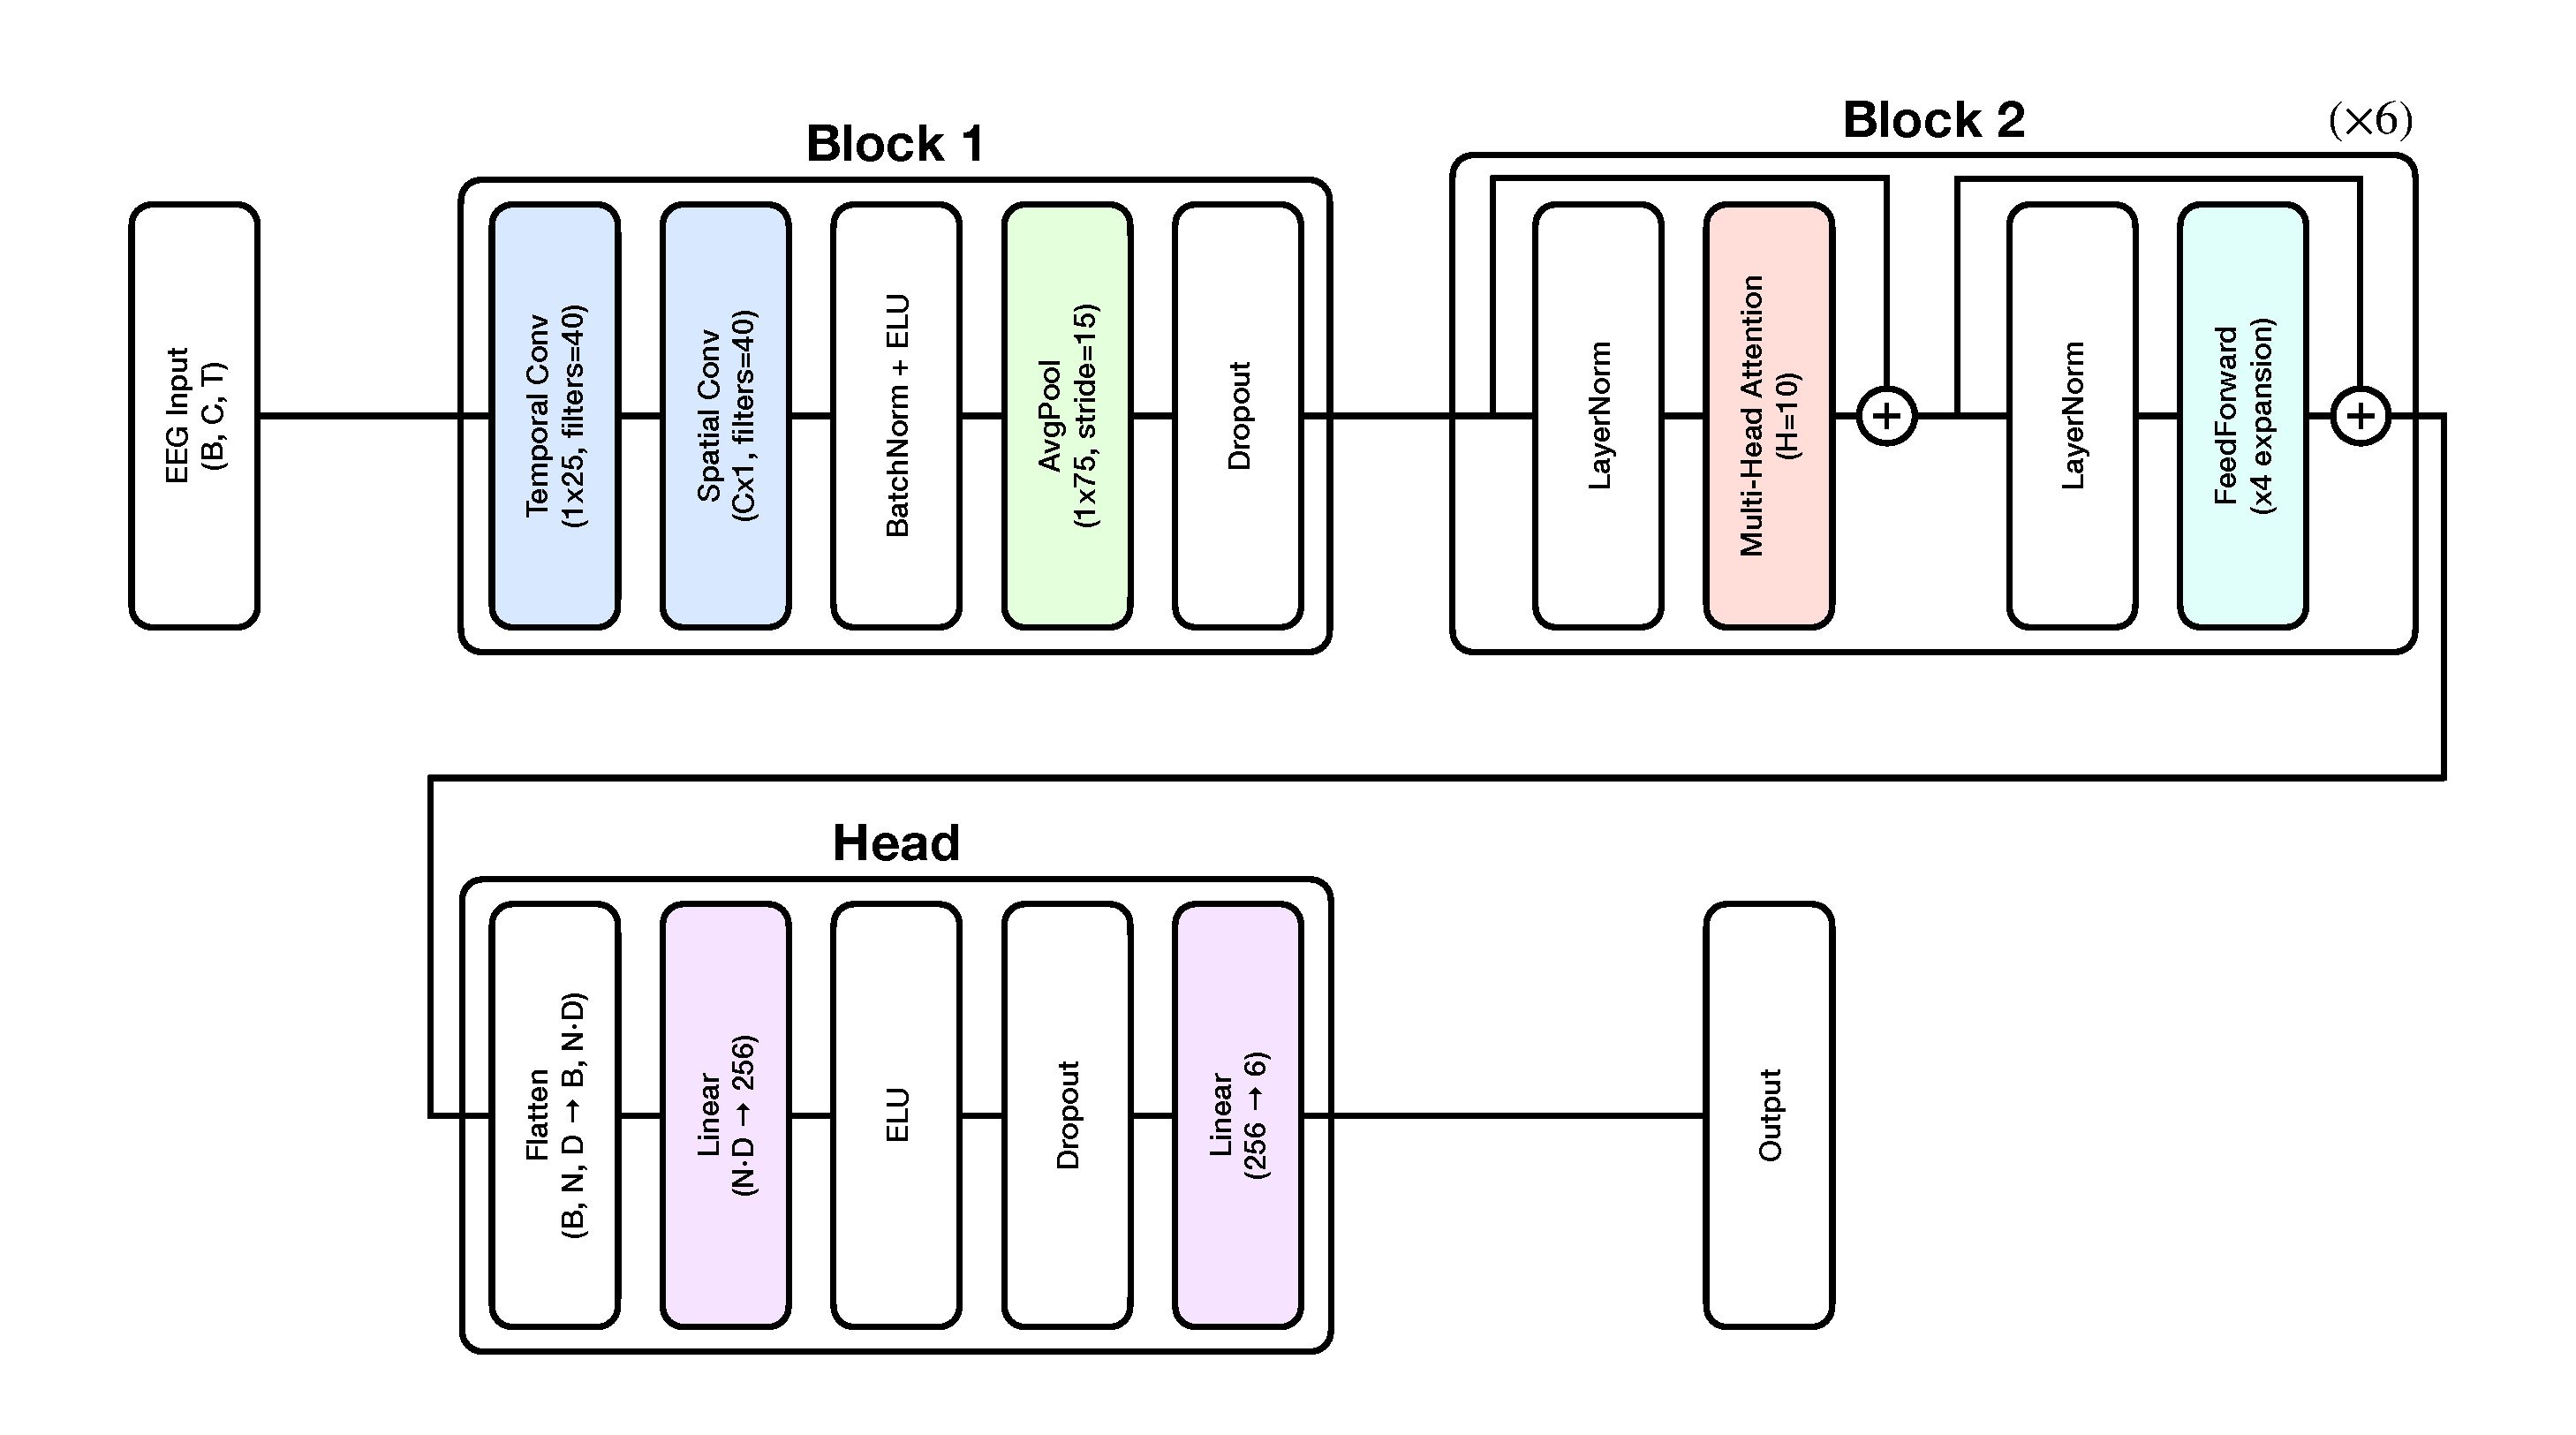
\includegraphics[width=1\textwidth]{images/EEGConformer.pdf}
    \caption{EEGConformer model structure showing Block 1 (temporal and spatial convolutional extraction), Block 2 (multi-head self-attention and feed-forward modeling), and Head (classification output).}
    \label{fig:EEGConformer}
\end{figure}

\chapter{Methodology}
\label{chap:methodology}

\section{Data Preparation and Splitting Strategy}

In this section the preprocessing steps and splitting strategy are introduced. In EEG classification tasks it is important to describe the steps of data preparation for both reproducibility and result interpretability. In this study the preprocessing pipeline is implemented with the goal of accurately simulating clinical practices.

\subsection{Data Preprocessing}

Before data analysis, model training, and experimentation, the raw data undergoes multiple preprocessing steps. 

\begin{description}

\item[\textbf{Removal of Constant Signal Edges:}] Some recordings contain segments where all signals are flat. These segments typically occur at the start or end of sessions and are easy to detect. During this step, all identified constant segments are removed, while the trimmed time points are recorded and the annotations are adjusted accordingly.

\item[\textbf{Temporal filtering and line-noise removal:}] Filtering changes the signal by mathematically removing unwanted parts that are in specific frequency ranges, as they are usually noise or drift rather than brain activity. A high-pass filter is applied to remove very slow changes in the signal, often caused by electrode drift due to sweat, skin potentials, or movement. A low-pass filter is also applied to remove very fast components, originating from electrical noise and muscle activity. Recordings contain a special hum-like noise from the power grid. A notch filter removes the narrow frequency band around the detected line-noise frequency, without removing the rest of the EEG spectrum.

\item[\textbf{Sampling rate validation and resampling:}] This is a simple frequency standardisation step, in which the original sampling rate of each file is checked, and if it differs from the default 250 Hz, the signal is resampled to the target rate.

\item[\textbf{Montage construction:}] The electrode signals contained in the raw EEG files are used to construct a standard set of channels, called a montage. In this specific pipeline, an average reference montage was constructed by calculating the difference between each electrode and the average of all electrodes.

\[
\tilde{x}_i(t) = x_i(t) - \frac{1}{N} \sum_{j=1}^{N} x_j(t)
\]

$x_i(t)$: electrode $i$ signal; $N$: number of electrodes; $\tilde{x}_i(t)$: average-referenced signal.

\item[\textbf{Amplitude scaling and clipping:}] Amplitudes of different EEG recordings may vary due to different amplifiers and hardware settings. For each recording, a scale factor was calculated from the middle 50\% of the absolute amplitude distribution, and global normalisation was performed, reducing sensitivity to outliers while standardising amplitude ranges across subjects and sessions. After scaling extreme EEG values were further suppressed by clipping signal amplitudes symmetrically to a threshold.

\item[\textbf{Composite label decomposition:}]

The original annotations of the TUAR dataset include composite labels like \texttt{eyem\_musc}, that represents recording segments where \texttt{eyem} and \texttt{musc} artifacts are both present. These classes are decomposed into overlapping base-label annotations to support multi-label learning. 

\item[\textbf{Z-score normalisation:}] The dataloader uses fixed-length, overlapping windows of a few seconds to segment the recordings, ensuring a consistent input representation for the models. For each window, per-channel z-score normalisation is applied to make sure all channels are on a similar scale providing consistency for the model. 

For a given window $x \in \mathbb{R}^{C \times T}$, where $C$ is the number of channels and $T$ is the number of time samples, the normalisation is defined as:

\[
z_{c,t} = \frac{x_{c,t} - \mu_c}{\sigma_c + \epsilon}
\]

$\mu_c$ and $\sigma_c$ are the average and standard deviation of channel $c$, and $\epsilon$ is a small constant added for stability.

This local normalisation prevents data leakage, helps stable training, and provides better numerical conditioning while preserving local signal structures.

\end{description}

 Each window is assigned all labels corresponding to artifact events that occur within its time interval. The preprocessing pipeline converts the raw EDF recordings into model-ready EDF files with standardised channel naming, consistent sampling rate, montage representation, amplitude normalisation, and time-aligned annotations.

\subsection{Dataset Splitting}

There are two problems with traditional dataset splitting techniques in case of window based EEG datapoints. The first one is data/patient leakage. By randomly assigning each datapoint to a split, many signal segments are going to end up in multiple splits due to the overlap of the constructed windows. In addition, patient-specific characteristics such as scalp geometry and individual brain rhythm patterns learned by the model will give unrealistic advantage in classifying the evaluation split, which misrepresents real expected performance of the model on new patients. To prevent this a patient-wise splitting technique is required. The second problem is the class imbalance in the dataset. By conducting a greedy splitting strategy, we would allow some classes to end up in a single split, which would make it impossible to train or evaluate on that class. Because of this, three mechanism were incorporated into the splitting mechanism:

\begin{description}

\item[\textbf{Patient-wise partitioning:}] Patient IDs are extracted and listed using the names of the EDF files. The files belonging to one particular patient are considered as one entity, which gets assigned to one particular split. As a result, all windows coming from the same patient get assigned to the same set, ensuring no leakage between splits.

\item[\textbf{Duration-weighted greedy assignment:}] For each patient a weight is calculated that represents the total recording time, sum of all EDF file durations in seconds of the corresponding patient. Patients are sorted from longest to shortest and assigned to the split that has its current total the furthest below its target duration. This greedy algorithm minimises the imbalance across splits.

\item[\textbf{Per-label balance objective:}] After the initial assignment, a local search performs pairwise patient swaps between the splits. A candidate swap is accepted if it decreases the total cost, where the cost is calculated using the combination of time balance error and label balance error. Time balance error is the relative squared deviation of total split duration from the target, while the label balance error is the sum, over all artifact classes, of the relative squared deviations between the annotated union duration of that class in each split and the desired class distribution across the splits. 
\newline.

\[
C = \sum_{s \in S} \left(\frac{T_s - T_s^{*}}{T_s^{*}}\right)^2
+ \alpha \sum_{l \in L} \sum_{s \in S} \left(\frac{D_{l,s} - D_{l,s}^{*}}{D_{l,s}^{*}}\right)^2
\]
\newline.

$S$ denotes the set of splits and $L$ the set of artifact labels. $T_s$ is the total recording duration of split $s$, with target duration $T_s^{*}$. $D_{l,s}$ is the annotated union duration of label $l$ in split $s$, and $D_{l,s}^{*}$ is its desired duration according to the target class distribution. The parameter $\alpha$ controls the relative importance of label balance.

This procedure iteratively improves the assignment, resulting in splits that are balanced in both total duration and artifact class representation.

\end{description}

The statistics of these optimised splits are presented in Table~\ref{tab:dataset_splits}.

\begin{table}[h]
\centering
\begin{tabular*}{\textwidth}{@{\extracolsep{\fill}}lcccc}
\toprule
\textbf{Split} & \textbf{Patients} & \textbf{Files} & \textbf{Total time} & \textbf{\% of total} \\
\midrule
Train & 182 & 235 & 75h 21m & 81.718\% \\
Dev   & 10  & 25  & 8h 27m  & 9.175\% \\
Test  & 9   & 30  & 08h 23m & 9.107\% \\
\midrule
Total & 201 & 290 & $\sim$92h & 100\% \\
\bottomrule
\end{tabular*}
\caption{Summary of dataset splits.}
\label{tab:dataset_splits}
\end{table}

\newpage

\section{Proposed  Latent Diffusion-Based Augmentation Method}

The proposed method is a latent diffusion-based synthetic data generation pipeline with similar core idea to the WGAN-GP. In the pipeline, a latent diffusion model (LDM) \cite{rombach2022} is trained to generate statistically similar datapoints to the real EEG windows from the TUAR dataset. 

For each artifact class, a separate model is used. This approach allows the models to specialise in the characteristics of a single artifact, rather than forcing a single model to learn conditional generation. The tradeoff is increased training time, memory usage, and required computational power in return for more realistic and accurate synthetic samples. During training, all datapoints corresponding to the given class are used, including the ones with multiple labels assigned. It is often considered better than using windows containing a single artifact because it avoids discarding many training samples and helps the model learn a more realistic and diverse representation of the data distribution.

In the LDM, a variational autoencoder (VAE) is combined with a denoising diffusion probabilistic model (DDPM), where first the compressed latent representation of EEG windows is learned by the VAE and then the diffusion model is trained to generate samples in this latent space. This low dimensional latent space allows the DDPM to use fewer denoising steps and maintain a lighter architecture, resulting in more efficient training and sampling. The diffusion model is trained to transform a sampled noise drawn from a gaussian distribution into a structured latent representation that reflects the learned data distribution. To achieve this, a denoising process over multiple timesteps is applied, where the model predicts and subtracts the noise component present in a given sample. Through this procedure, the model learns to reverse the forward diffusion process and generate coherent latent representations that can be decoded by the VAE into realistic EEG windows.

\subsection{Variational Autoencoder}

\subsubsection{Encoder}


First the encoder compresses the input EEG window $x \in \mathbb{R}^{B \times C \times T}$ into a low dimensional latent representation $h_\textbf{enc}  \in \mathbb{R}^{B \times C_\text{enc} \times T_\text{enc}}$ using a series of blocks each containing a 1D convolution layer with stride 2, group normalisation, and a SiLU activation function. 

\[
x \xrightarrow{\;\text{Conv + Norm + SiLU}\;} \ldots \xrightarrow{\;\text{Conv + Norm + SiLU}\;} h_\textbf{enc} 
\]

Then 1$\times$1 convolution is applied to $h$, and the tensor is split along the channel dimension to produce a Gaussian distribution for each latent variable.

\[
h_\textbf{enc}  \xrightarrow{\;\text{Conv + Split}\;} (\mu, \log \sigma^2)
\]

Using Gaussian distributions in the latent space enables stochastic sampling, allowing the model to generate synthetic EEG signal representation. 

At this point the reparameterisation trick is applied to enable differentiability. Instead of directly sampling from the distribution $\mathcal{N}(\mu, \sigma^2)$ the latent variable is redefined as: 

\[
z = \mu + \sigma \cdot \epsilon, \quad \epsilon \sim \mathcal{N}(0, I), \quad z \in \mathbb{R}^{B \times C_z \times T_z}
\]

where $\sigma = \exp\left(\frac{1}{2} \log \sigma^2 \right)$. This reformulation allows gradients to propagate through the sampling process during training.

\subsubsection{Decoder}

In the decoder the sampled latent representation $z$ is projected into a larger feature space by a 1$\times$1 convolution, where only the number of channels is modified, leaving the temporal length unchanged. 

\[
z  \xrightarrow{\;\text{Conv}\;} h_0, \qquad h_0 \in \mathbb{R}^{B \times C_d \times T_z}
\]

The decoder then applies a sequence of reconstruction blocks, where the input is upsampled with scale factor 2, followed by a convolution, group normalisation, and a SiLU activation function. 

\[
h_0 \xrightarrow{\;\text{Upsample + Conv + Norm + SiLU}\;} \ldots \xrightarrow{\;\text{Upsample + Conv + Norm + SiLU}\;} h_\textbf{dec} 
\]

After the reconstruction blocks, a finale convolution layer maps the decoder feature representation back into the original EEG signal space.

\[
h_{\text{dec}} \xrightarrow{\;\text{Conv}\;} \hat{x}, \qquad \hat{x} \in \mathbb{R}^{B \times C \times T}
\]

This decoding process enables the reconstruction of EEG signals from compact latent representations, while preserving their temporal structure.

\subsubsection{Loss Function}

During training, the VAE has two main objectives: accurate reconstruction of the EEG signal and to regularise the latent space to follow a Gaussian distribution. To achieve this, the following loss function is used: 

\[
\mathcal{L}_{\text{VAE}} = \mathcal{L}_{\text{recon}} + \lambda_{\text{KL}} \mathcal{L}_{\text{KL}}
\]

$\mathcal{L}_{\text{recon}}$ can be either L1 or MSE:

\[
\begin{aligned}
\text{L1:} \quad & \mathcal{L}_{\text{recon}} = \frac{1}{N} \sum_{i=1}^{N} |x_i - \hat{x}_i| \\
\text{MSE:} \quad & \mathcal{L}_{\text{recon}} = \frac{1}{N} \sum_{i=1}^{N} (x_i - \hat{x}_i)^2
\end{aligned}
\]

The KL divergence loss $\mathcal{L}_{\text{KL}}$ enforces $\mu \approx 0$ and $\sigma^2 \approx 1$ in the following way:

\[
\mathcal{L}_{\mathrm{KL}} = -\frac{1}{2} \sum \left( 1 + \log \sigma^2 - \mu^2 - \sigma^2 \right)
\]

The weight $\lambda_{\text{KL}}$ controls the importance of the KL divergence term in the total loss. These loss components together help the model learn both reconstruction and structured latent space representation.

\subsection{Latent Diffusion}

\subsubsection{Training}

The input of the diffusion model $z$ is the latent representation of an EEG window produced by the VAE. $z$ is scaled to have its variance normalized, because diffusion models assume inputs with approximately unit variance. 

\[
z \xrightarrow{\;\text{Scaling}\;} \tilde{z}
\]

After the scaling, a diffusion timestep $t$ is uniformly sampled from the set $\{0, \dots, T-1\}$ and Gaussian noise $\epsilon$ is generated.

\[
t \sim \mathcal{U}(0, T-1), \qquad \epsilon \sim \mathcal{N}(0, I)
\]

Using the sampled timestep and noise, along with the precomputed cumulative product of the diffusion coefficients $\bar{\alpha}_t$, the forward diffusion process corrupts the latent representation. 

\[
z_t = \sqrt{\bar{\alpha}_t}\, \tilde z + \sqrt{1 - \bar{\alpha}_t}\, \epsilon
\]

For a small $t$ value, the signal-to-noise ratio is high, but as $t$ increases, the ratio gradually decreases. 

The returned noisy tensor $z_t$ and the determined timestep scalar $t$ are passed to the denoising network. A higher dimensional vector representation of $t$ is computed using sinusoidal positional encoding. The sinusoidal embedding is passed through an MLP, consisting of two linear layers and an SiLU activation function. 

\[
t \xrightarrow{\;\text{Sinusoidal embedding}\;} \gamma(t) \xrightarrow{\;\text{MLP}\;} e_t
\]

The noisy latent tensor and the time embedding vector are given to a 1D U-Net. This denoising network consists of a downsampling path with residual blocks conditioned on the timestep, a bottleneck, and a symmetric upsampling path with skip connections. The output of the U-Net is the predicted noise component $\epsilon_\theta(z_t, e_t)$ of the input $z_t$.

\[
(z_t, e_t) \xrightarrow{\text{U-Net}} \epsilon_\theta(z_t, e_t)
\]

The goal of the training is to minimise the mean squared error between the predicted and true noise.

\[
\mathcal{L}_{\text{diff}} = \mathbb{E} \left[ \left\| \epsilon_\theta(z_t, e_t) - \epsilon \right\|^2 \right]
\]

During diffusion training, the parameters of the U-Net and the sinusoidal embedding MLP are changed, while the weights of the VAE remain fixed.

\subsubsection{Synthetic Data Generation}

In order to generate synthetic EEG windows, we need to sample from the latent distribution using the reverse diffusion process, and then transform it to a synthetic window through the decoder. The process starts with an initial Gaussian noise sample in the latent space: 

\[
z_T \sim \mathcal{N}(0, I), \qquad z_T \in \mathbb{R}^{B \times C_z \times T_z}
\]

where $z_T$ represents the corrupted latent sample at the final diffusion timestep $T$.

The model iteratively refines the latent representation by  predicting the noise component of the current latent tensor $z_t$, and estimating a less noisy latent representation at the previous timestep.

\[
(z_t, e_t) \xrightarrow{\text{U-Net}} \epsilon_\theta(z_t, e_t)
\]

\[
z_{t-1} = \frac{1}{\sqrt{\alpha_t}} \left( z_t - \frac{\beta_t}{\sqrt{1 - \bar{\alpha}_t}} \, \epsilon_\theta(z_t, e_t) \right) + \sigma_t \cdot \eta
\]

where $\beta_t$ and $\alpha_t$ are diffusion coefficients, $\sigma_t$ controls the noise scale, and $\eta \sim \mathcal{N}(0, I)$ is Gaussian noise.

After the last diffusion step $t = 0$, the final latent representation $z_0$ is rescaled to match the original latent distribution and passed to the VAE decoder, which reconstructs the final synthetic EEG window.

\[
z_0 \xrightarrow{\;\text{Unscaling}\;} \hat{z} \xrightarrow{\;\text{VAE Decoder}\;} \hat{x}, \qquad \hat{x} \in \mathbb{R}^{B \times C \times T}
\]

This method enables the synthesis of realistic EEG signals by first sampling in the structured latent space and then reconstructing them in the original signal domain.

\subsection{Overview}

The proposed method is to use this latent diffusion-based generative approach to produce fully synthetic data, add it to the original dataset, and measure the effect on artifact classification. First, the VAE is trained to learn the representation of EEG data in the latent space, then the diffusion model is trained in the latent space to model the distribution of the encoded representations. For each class, a separate model is trained to allow label specialisation. 

For the augmentation set used in training classification models, a new method is added that uses the trained LDMs for synthetic data generation. This approach enables the generation of diverse and realistic synthetic samples, which is expected to improve robustness and generalisation.

\begin{figure}[H]
\centering
    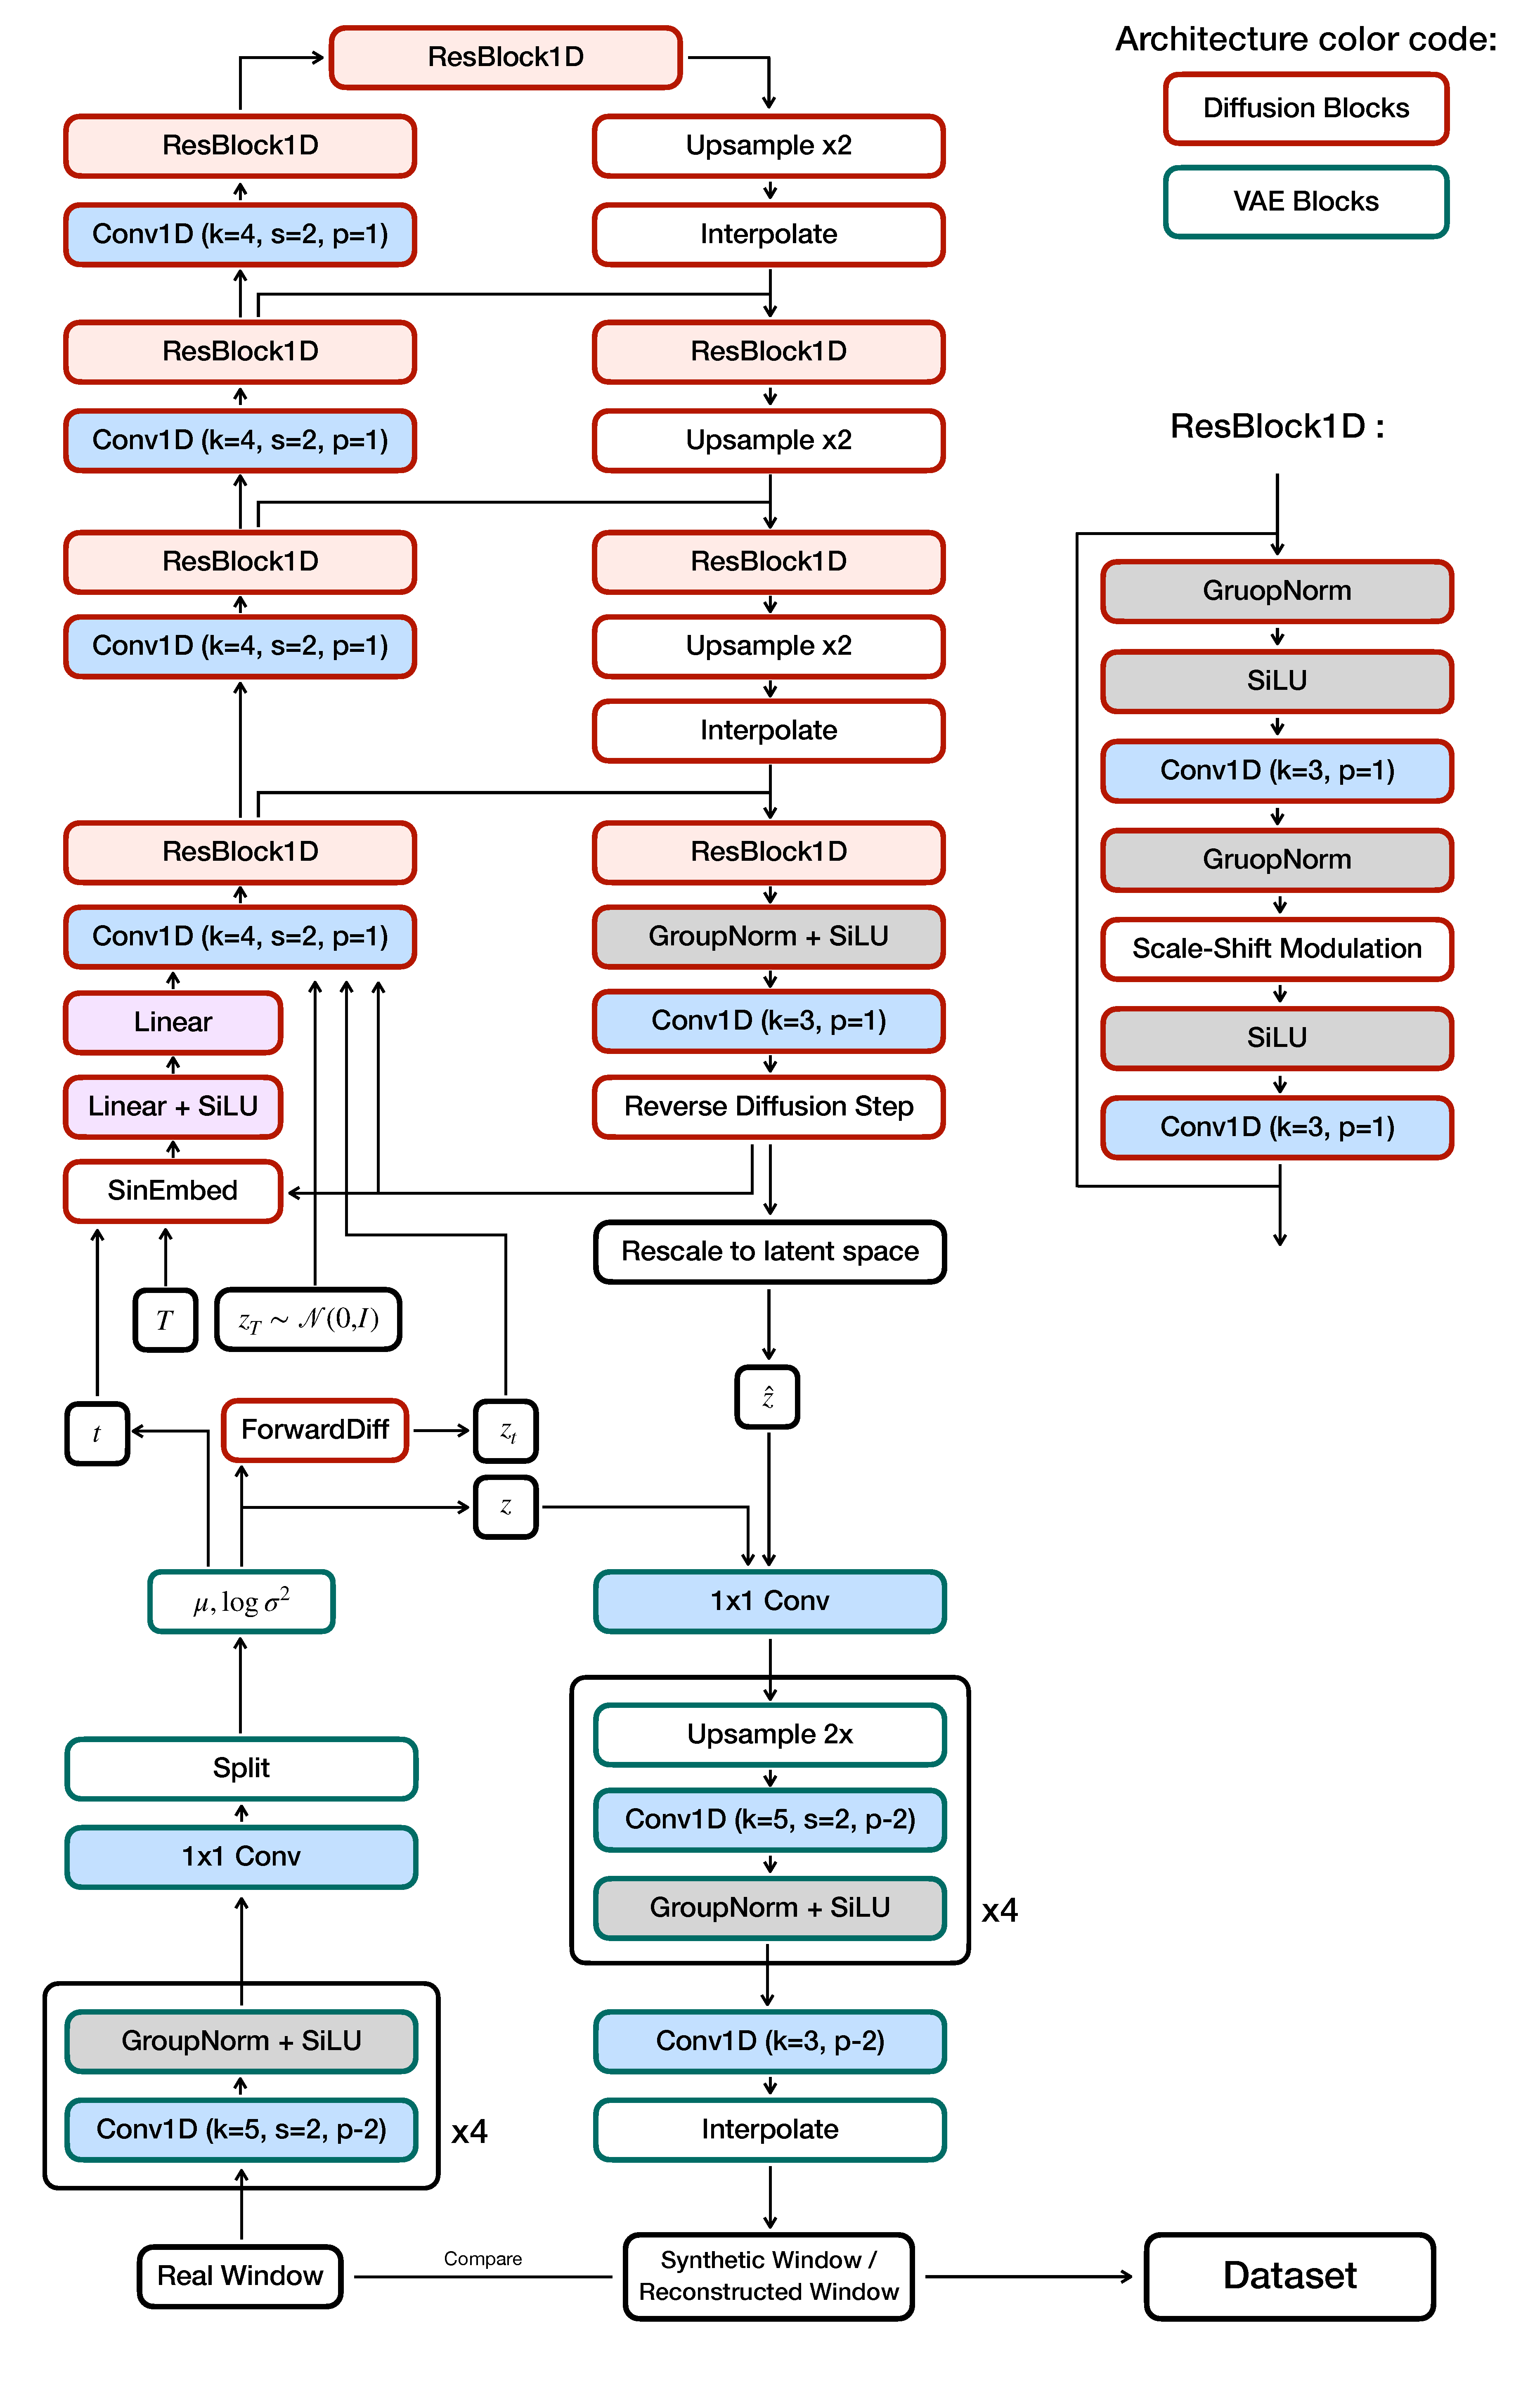
\includegraphics[width=0.9\textwidth]{images/LDM.pdf}
    \caption{Latent diffusion architecture for EEG signal generation. The VAE encodes the input $x$ into a latent $z$, which is corrupted to $z_t$ via forward diffusion. A 1D U-Net predicts and removes noise conditioned on the timestep, producing $\hat{z}$, which is decoded into the reconstructed signal $\hat{x}$.}
    \label{fig:LDM}
\end{figure}

\newpage

\section{Evaluation Metrics}

\subsection{Macro F1}

The primary metric for evaluating model performance is Macro F1-score in this study. This metric is particularly suitable for imbalanced datasets, such as TUAR, as it equally represents the contribution of minor classes and prevents dominance by majority labels. For a single class $c$, it is defined as:

\[
F1_c = \frac{2 \cdot \mathrm{Precision}_c \cdot \mathrm{Recall}_c}{\mathrm{Precision}_c + \mathrm{Recall}_c}
\]

\[
\text{Precision}_c = \frac{TP_c}{TP_c + FP_c}, \quad
\text{Recall}_c = \frac{TP_c}{TP_c + FN_c}
\]

Macro F1 is computed as the unweighted mean of the per-class F1-scores:

\[
\text{Macro F1} = \frac{1}{C} \sum_{c=1}^{C} F1_c
\]

This makes Macro F1 an accurate indicator of overall performance under class imbalance.

\subsection{Macro PR AUC}

Macro PR AUC is the secondary metric for evaluating model performance. While the F1-score evaluates using a single threshold, PR AUC measures all possible thresholds and reflects the ranking quality of the model.

For each artifact class, the PR AUC is computed separately, where each label is treated as an independent binary classification task. For class $c$, confidence scores are computed and a PR curve is constructed by varying the decision threshold.

The Macro PR AUC is defined as:

\[
\text{Macro PR AUC} = \frac{1}{C} \sum_{c=1}^{C} \text{PR AUC}_c
\]

Where $\text{PR AUC}_c$ is the area under the PR curve for class $c$.
Macro PR AUC is an informative metric in imbalanced settings, where negative samples can dominate.\\

\textbf{Additional Metrics}

Precision, recall, F1-score, and PR AUC were also monitored for performance evaluation.

\section{Experimental Design and Parameter Selection}

\subsection{Data Preparation}

\subsubsection{Window length}

Selecting the length of the EEG window is an important design decision. Shorter windows allow the model to detect short artifacts but may lack information for accurate classification. Larger window size improves the detection of longer and more complex EEG patterns but makes it harder to localise short events. The EEG recordings were sampled at 250~Hz.

To select the appropriate window length, experiments were conducted. All five classification models were trained using different window sizes. The parameter with the best metrics averaged across all models was selected. 

\begin{table}[H]
\centering
\begin{tabular}{c}
\toprule
\textbf{Evaluated window sizes (s)} \\
\midrule
1 \\
2 \\
4 \\
6 \\
\textbf{8}\\
10 \\
\bottomrule
\end{tabular}
\end{table}

The selected window size for subsequent experiments is 8~s.

\subsubsection{Stride}

The stride parameter determines the overlap between two consecutive windows. Smaller stride results in repeated samples and an increased number of windows extracted from the signal, which helps compensate imbalanced data. To determine the setting, a similar experiment was conducted as in the window size optimisation. 

\begin{table}[H]
\centering
\begin{tabular}{c}
\toprule
\textbf{Evaluated stide settings (s)} \\
\midrule
\textbf{0.5} \\
1 \\
2 \\
4 \\
\bottomrule
\end{tabular}
\end{table}

Stride of 0.5 s was selected based on the results.

\subsubsection{Sampling rate handling}

During training, a two-stage sampling strategy was used. In the first epoch, all samples were observed once, and the repeat factor of each class was calculated based on their frequencies. For the remaining epochs, the selection probabilities increased in proportion to the repeat factor of the corresponding class. The repeat factor for class $c$:

\[
r_c = \sqrt{\frac{1}{f_c}}
\]

where $f_c$ is the frequency of the given class.

Using this sampling method, the model is exposed more frequently to rare classes, which helps avoid class dominance.

\subsection{Model and Training Configuration}

\subsubsection{Batch size and learning rate}

To ensure a controlled experimental setup and isolate the effect of augmentation methods, the same batch size and learning rate were used for all classification models. These were selected by conducting multiple experiments on all models with different hyperparameter settings. The metrics were averaged across models and the parameters were selected based on the results.

\begin{table}[H]
\centering

\begin{minipage}{0.45\textwidth}
\centering
\begin{tabular}{c}
\toprule
\textbf{Evaluated batch size} \\
\midrule
32 \\
\textbf{64} \\
128 \\
256 \\
\bottomrule
\end{tabular}
\end{minipage}
\hfill
\begin{minipage}{0.45\textwidth}
\centering
\begin{tabular}{c}
\toprule
\textbf{Evaluated learning rate} \\
\midrule
$1 \times 10^{-3}$ \\
$3 \times 10^{-4}$ \\
$\mathbf{1 \times 10^{-4}}$ \\
$5 \times 10^{-5}$ \\
$1 \times 10^{-5}$ \\
\bottomrule
\end{tabular}
\end{minipage}

\end{table}

Selected parameters: batch size = 64, learning rate: $1 \times 10^{-4}$


\subsubsection{Number of epochs}

In order to determine the length of the training, an additional experiment was conducted in which all models were trained for an extended 200 epochs and the peak performance of each model was monitored. The top metrics were achieved before 40 epochs for each model. 

Based on these results, 100 epochs were selected as the final training parameter.

\subsubsection{Optimizer}

The AdamW optimizer was used for the conducted experiments in this thesis. The usage of adaptive learning rates and decoupled weight decay makes it ideal for training deep neural networks where regularisation and stable convergence are important. 

\subsubsection{Loss Function}

To handle class imbalance, Asymmetric Loss (ASL) was used as the main loss function. Let $z$ denote the predicted logit, $p$ the predicted probability, and $y \in \{0,1\}$ the target label. The loss is defined as

\[
\mathcal{L}_{\text{ASL}} = - \left[ y \log(p) + (1 - y)\log(\tilde{p}^{-}) \right] (1 - p_t)^\gamma,
\]

where $\tilde{p}^{-} = \min(1 - p + c, 1)$ is the clipped negative probability, and $p_t$ is defined as $p_t = p$ if $y = 1$, and $p_t = 1 - p$ otherwise.

Different focusing parameters are applied to positive and negative samples, making the loss asymmetric. This reduces the influence of easy negative examples and improves learning for rare classes. In this work, $\gamma_{+} = 1.0$, $\gamma_{-} = 2.0$, and $c = 0.05$ were used.

\subsection{Augmentation Settings}

\subsubsection{Non-generative augmentation parameters}

The selected parameters follow commonly used practices in EEG signal processing. These augmentation settings introduce controlled perturbations which help improve model generalisation and preserve the characteristics of the signal.

\begin{table}[H]
\centering
\label{tab:augmentation_defaults}

\begin{tabularx}{\textwidth}{l X l}
\toprule
\textbf{Augmentation} & \textbf{Parameters} & \textbf{Values} \\
\midrule
Gaussian noise           & Probability, SNR                    & 0.5, 20 dB \\
Pink noise        & Probability, SNR                    & 0.5, 20 dB \\
Temporal augmentations & Crop fraction, shift fraction       & 0.9, 0.05 \\
Segment recombination & Probability, number of segments     & 0.5, 8 \\
Channel dropout       & Probability, dropped channel fraction & 0.5, 0.1 \\
Mixup-style blending  & Probability, signal/noise ratio     & 0.5, 0.9 / 0.1 \\
\bottomrule
\end{tabularx}
\end{table}

\newpage

\subsubsection{Generative augmentation parameters}

A series of experimental trainings have been conducted in order to optimize  the hyperparameters of the generative augmentation techniques. Both the WGAN-GP and the LDM required different epoch settings for major and minor classes due to the different number of datapoints corresponding to the given label.The selected parameters are shown in the table below.

\begin{table}[H]
\centering
\begin{tabular*}{\textwidth}{@{\extracolsep{\fill}}lccc}
\toprule
\textbf{Model} & \textbf{WGAN-GP} & \textbf{VAE} & \textbf{LDM} \\
\midrule
Batch size     & 32     & 32     & 32 \\
Learning rate  & $2\times10^{-4}$ & $1\times10^{-3}$ & $2\times10^{-4}$ \\
Epoch-major    & 50     & 50     & 150 \\
Epoch-minor    & 500    & 200    & 2000 \\
Optimizer      & Adam   & Adam   & Adam \\
\bottomrule
\end{tabular*}
\end{table}

After the hyperparameter optimisation both models were trained on each class and saved for later integration into the augmentation pipeline.

\subsection{Experiments and Notation}

Two comprehensive experiments were conducted. In the first, each model–augmentation pair was trained multiple times and the average performance was measured for all pairs. The purpose of this experiment was to measure how much performance gain can be achieved using the diffusion-based method compared to baseline augmentations. By using multiple EEG classification models and conducting several trainings for each model–augmentation pair we can get wider picture of the potential of the proposed method.

The second experiment compared two existing augmentation pipelines and their combinations with two generative augmentation methods. Because augmentations are rarely used alone, it is important to test the proposed method by combining it with other techniques. The result of this experiment demonstrates the true potential of using latent diffusion-based augmentation for enhancing classification performance.

Table \ref{tab:augmentation_abbreviations} shows the set of augmentations used in the experiments and their notations for later analysis. The classification models are described in Chapter \ref{chap:background}.

\begin{table}[H]
\centering
\footnotesize
\setlength{\tabcolsep}{0pt}
\renewcommand{\arraystretch}{1.08}

\begin{tabular}{l@{\hspace{6em}}l}
\toprule
\textbf{Abbreviation} & \textbf{Method} \\
\midrule
BASE & No augmentation \\
GAUS & Gaussian noise \\
PINK & Pink noise \\
TEMP & Temporal augmentations \\
SEGR & Segment recombination \\
CHDO & Channel dropout \\
MIXU & Mixup-style blending  \\
WGAN & WGAN-GP-based generation \\
LDIF & Latent diffusion-based augmentation \\
\midrule
\multirow{2}{*}{CAP} & Composite Augmentation Pipeline \\
                     & \hspace{1.5em}PINK, TEMP, CHDO, MIXU \\
\addlinespace[3pt]
\multirow{2}{*}{CPP} & Signal Perturbation Pipeline \\
                     & \hspace{1.5em}GAUS, TEMP, SEGR \\
\bottomrule
\end{tabular}

\caption{Summary of the abbreviations used in the Results section for augmentation methods and composite pipelines.}
\label{tab:augmentation_abbreviations}
\end{table}

The Composite Augmentation Pipeline (CAP) combines pink noise injection and temporal augmentation methods with channel dropout and window blending techniques. Signal Perturbation Pipeline (CPP) replaces pink noise with Gaussian noise and combines it with segment recombination, while also including the temporal augmentation. 

Generative augmentations were combined with these pipelines with the goal of measuring their ability to further improve existing pipelines and to compare the effectiveness of the proposed latent diffusion-based method with WGAN-GP-based generation.

\subsection{Framework and Hardware}

\begin{itemize}
    \item Language and environment: Python 3.12 (conda)
    \item EEG processing framework: MNE-Python
    \item Deep learning framework: PyTorch 2.10.0
    \item CUDA: 12.8
    \item Data format: European Data Format (EDF)
\end{itemize}

All experiments were conducted on an NVIDIA GeForce RTX 2080 Ti GPU (11 GB VRAM) available on the server gpu01.cs.elte.hu provided by the Institute of Mathematics, Eötvös Loránd University.

\chapter{Results}
\label{chap:results}

\section{Augmentation Results}

\begin{table}[H]
\centering
\setlength{\tabcolsep}{4pt}
\renewcommand{\arraystretch}{1.25}
\scriptsize
\resizebox{\textwidth}{!}{%
\begin{tabular}{lccccccccc}
\toprule
\textbf{Model} & \textbf{BASE} & \textbf{GAUS} & \textbf{PINK} & \textbf{TEMP} & \textbf{SEGR} & \textbf{CHDO} & \textbf{MIXU} & \textbf{WGAN} & \textbf{LDIF} \\
\midrule

EEGNet 
& \makecell{0.6781 \\ 0.6330}
& \makecell{0.6795 \\ 0.6295}
& \makecell{0.6982 \\ 0.6499}
& \makecell{0.6858 \\ 0.6432}
& \makecell{\textbf{0.7072} \\ 0.6521}
& \makecell{0.6984 \\ 0.6459}
& \makecell{0.6941 \\ \textbf{0.6577}}
& \makecell{0.7001 \\ 0.6510}
& \makecell{0.6993 \\ 0.6475} \\
\midrule

EEGNeX
& \makecell{0.7164 \\ 0.6586}
& \makecell{0.7191 \\ 0.6585}
& \makecell{0.7354 \\ 0.6757}
& \makecell{0.7348 \\ 0.6778}
& \makecell{\textbf{0.7489} \\ \textbf{0.6874}}
& \makecell{0.7358 \\ 0.6601}
& \makecell{0.7361 \\ 0.6779}
& \makecell{0.7443 \\ 0.6806}
& \makecell{0.7435 \\ 0.6821} \\
\midrule

EEGInceptionERP
& \makecell{0.6568 \\ 0.6163}
& \makecell{0.6584 \\ 0.6245}
& \makecell{0.6720 \\ 0.6305}
& \makecell{0.6683 \\ 0.6303}
& \makecell{\textbf{0.6896} \\ \textbf{0.6420}}
& \makecell{0.6835 \\ 0.6319}
& \makecell{0.6780 \\ 0.6364}
& \makecell{0.6827 \\ 0.6359}
& \makecell{0.6809 \\ 0.6367} \\
\midrule

CNN-LSTM
& \makecell{0.7145 \\ 0.6510}
& \makecell{0.7257 \\ 0.6595}
& \makecell{0.7318 \\ 0.6645}
& \makecell{0.7300 \\ 0.6778}
& \makecell{\textbf{0.7405} \\ \textbf{0.6792}}
& \makecell{0.7358 \\ 0.6688}
& \makecell{0.7352 \\ 0.6733}
& \makecell{0.7386 \\ 0.6761}
& \makecell{0.7394 \\ 0.6763} \\
\midrule

EEGConformer
& \makecell{0.6512 \\ 0.6214}
& \makecell{0.6629 \\ 0.6136}
& \makecell{0.6784 \\ 0.6419}
& \makecell{0.6726 \\ 0.6455}
& \makecell{\textbf{0.6862} \\ 0.6490}
& \makecell{0.6748 \\ 0.6446}
& \makecell{0.6779 \\ 0.6308}
& \makecell{0.6835 \\ \textbf{0.6492}}
& \makecell{0.6806 \\ 0.6489} \\
\midrule

Average
& \makecell{0.6834 \\ 0.6360}
& \makecell{0.6891 \\ 0.6371}
& \makecell{0.7031 \\ 0.6525}
& \makecell{0.6983 \\ 0.6549}
& \makecell{\textbf{0.7144} \\ \textbf{0.6619}}
& \makecell{0.7056 \\ 0.6502}
& \makecell{0.7042 \\ 0.6552}
& \makecell{0.7098 \\ 0.6585}
& \makecell{0.7087 \\ 0.6583} \\
\midrule

$\Delta$ (\%)
& \makecell{0 \\ 0}
& \makecell{0.83 \\ 0.17}
& \makecell{2.88 \\ 2.59}
& \makecell{2.18 \\ 2.97}
& \makecell{\textbf{4.53} \\ \textbf{4.07}}
& \makecell{3.24 \\ 2.23}
& \makecell{3.04 \\ 3.01}
& \makecell{3.86 \\ 3.53}
& \makecell{3.70 \\ 3.50} \\
\bottomrule
\end{tabular}%
}
\caption{Combined comparison of model performance across augmentation settings. Each cell reports Macro F1 (top) and Macro PR AUC (bottom).}
\label{tab:combined_aug_results}
\end{table}

The results of the model-augmentation paired trainings are presented in Table~\ref{tab:combined_aug_results}. Each cell contains the Macro F1 and Macro PR AUC metrics for the corresponding pair, where the values represent the average of three different training runs.

All augmentation methods were able to consistently improve performance compared to the baseline setup. For each model, both the Macro F1 and Macro PR AUC scores increased with the use of augmentations with the only exception being Gaussian noise injection, which showed occasional drops in Macro PR AUC values. Pink noise resulted in noticeably higher performance gain than gaussian noise augmentation. This indicates that pink noise is more effective than Gaussian noise in improving model performance in the evaluated setup.

The highest overall performance was acchieved by SEGR, with largest relative improvement compared to the baseline, +4.53\% in Macro F1 and +4.07\% in Macro PR AUC. 

The two generative method also led to notable improvements. WGAN and the proposed LDIF achieved strong gains of +3.86\% and +3.70\% Macro F1 respectively. WGAN even resulted in highest Macro PR AUC score for EEGConformer, while MIXU achieved the top score for EEGNet. 

On model level, the global best performance was achieved by the EEGNeX, reaching a Macro F1 score of 0.7489. On the other hand, EEGNet shows the lowest overall performance across all models. 

Figure~\ref{fig:augmentation_delta} further highlights augmentation effects by comparing the relative performance gains of each method. The comparison between Macro F1 and Macro PR AUC gains shows that certain augmentations, such as MIXU, WGAN and LDIF, managed to achieve relatively balanced improvements across both metrics. Additionally, the relatively small variability of multiple runs indicates the consistency of the augmentation effects.

While all augmentation techniques are able to improve model performance in general, the magnitude of improvements differ across methods. Although SEGR achieves the highest scores, the proposed LDIF method remains competitive and consistent across all models.

\begin{figure}[H]
\centering
    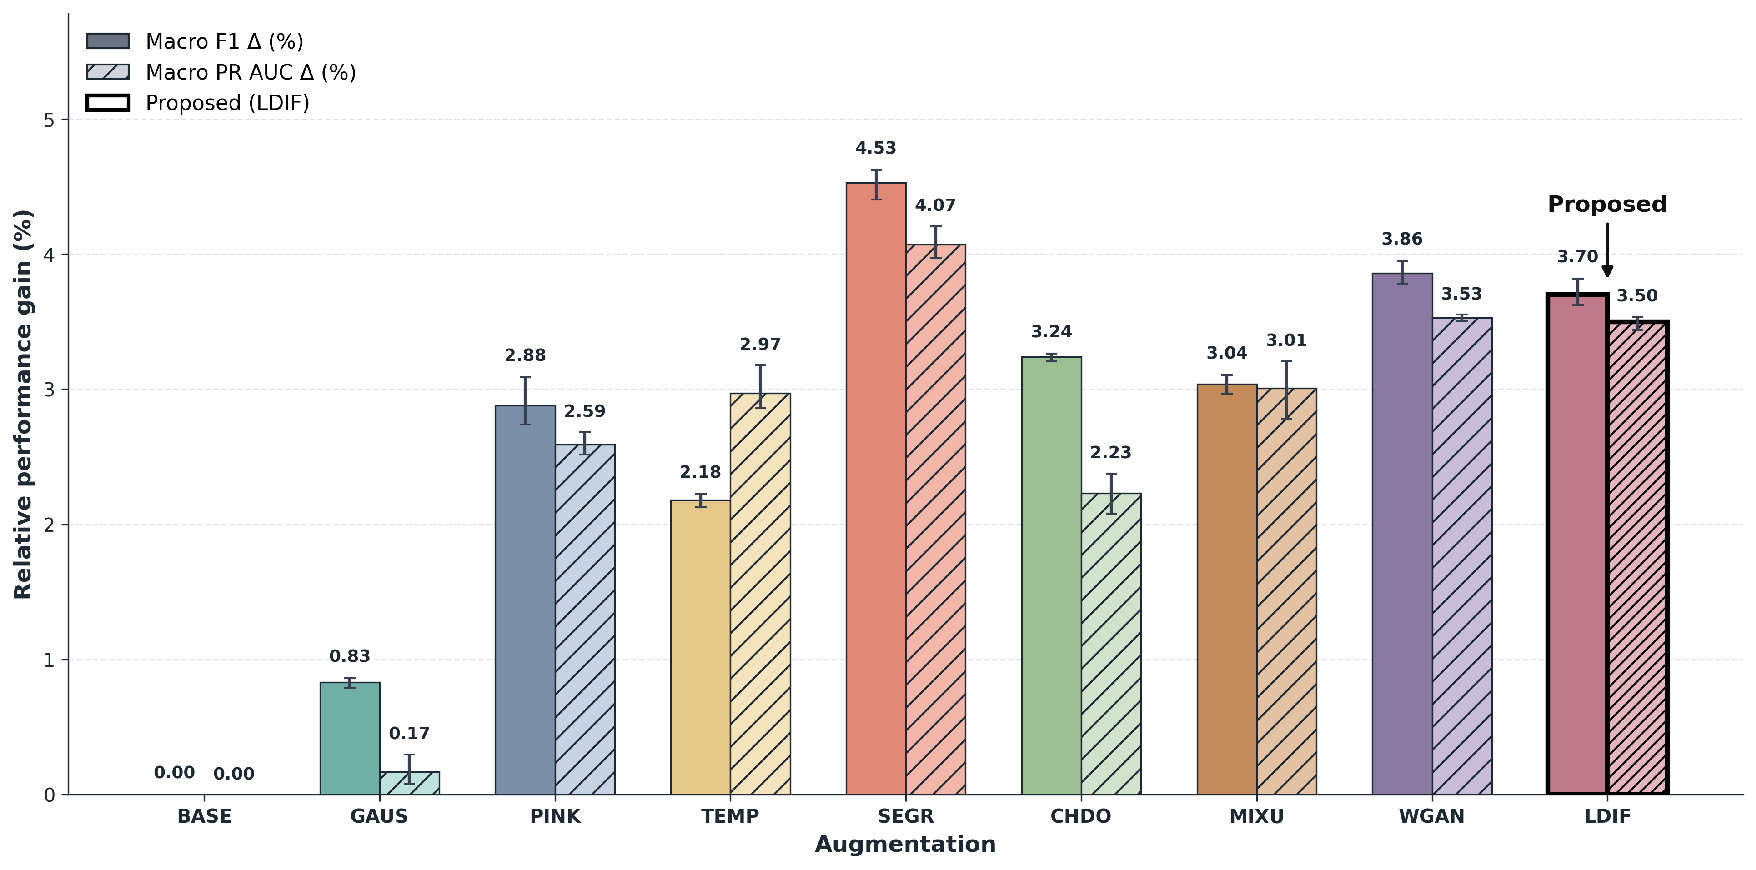
\includegraphics[width=1\textwidth]{images/augmentation_delta.pdf}
    \caption{Relative performance gains (\%) of augmentation methods compared to the baseline, measured in Macro F1 (solid) and Macro PR AUC (hatched). The proposed method (LDIF) is highlighted. Error bars indicate the min–max range across runs.}
    \label{fig:augmentation_delta}
\end{figure}

\section{Composition-Based Comparison}

\newcolumntype{C}[1]{>{\centering\arraybackslash}p{#1}}

\begin{table}[H]
\centering
\renewcommand{\arraystretch}{1.25}
\setlength{\tabcolsep}{3pt}

\resizebox{\textwidth}{!}{%
\begin{tabular}{@{}C{3cm}*{7}{C{2cm}}@{}}
\toprule
\textbf{Model} & 
\textbf{BASE} & 
\textbf{CAP} & 
\textbf{CPP} & 
\makecell{\textbf{CAP +}\\\textbf{WGAN}} & 
\makecell{\textbf{CPP +}\\\textbf{WGAN}} & 
\makecell{\textbf{CAP +}\\\textbf{LDIF}} & 
\makecell{\textbf{CPP +}\\\textbf{LDIF}} \\
\midrule

EEGNet
& \makecell{0.6781 \\ 0.6330}
& \makecell{0.7125 \\ 0.6609}
& \makecell{0.7089 \\ 0.6526}
& \makecell{0.7160 \\ 0.6658}
& \makecell{0.7143 \\ 0.6658}
& \makecell{\textbf{0.7175} \\ 0.6614}
& \makecell{0.7128 \\ 0.6598} \\
\midrule

EEGNeX
& \makecell{0.7164 \\ 0.6586}
& \makecell{0.7543 \\ 0.6846}
& \makecell{0.7498 \\ 0.6873}
& \makecell{\textbf{0.7555} \\ \textbf{0.6896}}
& \makecell{0.7486 \\ 0.6658}
& \makecell{0.7550 \\ 0.6860}
& \makecell{0.7510 \\ 0.6831} \\
\midrule

EEGInceptionERP
& \makecell{0.6568 \\ 0.6163}
& \makecell{0.6936 \\ 0.6487}
& \makecell{0.6907 \\ 0.6466}
& \makecell{\textbf{0.6977} \\ 0.6513}
& \makecell{0.6954 \\ 0.6507}
& \makecell{0.6924 \\ 0.6543}
& \makecell{0.6927 \\ \textbf{0.6612}} \\
\midrule

CNN-LSTM
& \makecell{0.7145 \\ 0.6510}
& \makecell{0.7491 \\ 0.6845}
& \makecell{0.7492 \\ 0.6824}
& \makecell{0.7481 \\ \textbf{0.6901}}
& \makecell{\textbf{0.7503} \\ 0.6880}
& \makecell{0.7481 \\ 0.6857}
& \makecell{0.7463 \\ 0.6828} \\
\midrule

EEGConformer
& \makecell{0.6512 \\ 0.6214}
& \makecell{0.6920 \\ 0.6548}
& \makecell{0.6919 \\ 0.6536}
& \makecell{0.6973 \\ \textbf{0.6589}}
& \makecell{\textbf{0.6954} \\ 0.6572}
& \makecell{0.6944 \\ 0.6561}
& \makecell{0.6920 \\ 0.6509} \\
\midrule

Average
& \makecell{0.6834 \\ 0.6360}
& \makecell{0.7203 \\ 0.6667}
& \makecell{0.7181 \\ 0.6645}
& \makecell{\textbf{0.7229} \\ \textbf{0.6711}}
& \makecell{0.7208 \\ 0.6655}
& \makecell{0.7214 \\ 0.6687}
& \makecell{0.7189 \\ 0.6675} \\
\midrule

$\Delta$ (\%)
& \makecell{0 \\ 0}
& \makecell{5.39 \\ 4.82}
& \makecell{5.07 \\ 4.48}
& \makecell{\textbf{5.77} \\ \textbf{5.51}}
& \makecell{5.47 \\ 4.63}
& \makecell{5.56 \\ 5.14}
& \makecell{5.19 \\ 4.95} \\
\bottomrule
\end{tabular}%
}
\caption{Combined comparison of model performance across combined augmentation settings. Each cell reports Macro F1 (top) and Macro PR AUC (bottom).}
\label{tab:combined_composition_results}
\end{table}

The results of the composition-based trainings are presented in Table~\ref{tab:combined_composition_results}. Similarly to the model-augmentation paired settings, all composition-based methods improved performance compared to the baseline across all models.

Both CAP and CPP further improved the scores compared to the previous experiment, corresponding to more than 5\% gains in Macro F1 and 4\% in Macro PR AUC score over the baseline. The introduction of generative augmentations improved upon these results, as the addition of both WGAN and LDIF increased the overall performance.

The combined method of CAP + WGAN resulted in the highest average performance gain, achieving +5.77\% in Macro F1 and +5.51\% in Macro PR AUC. While the addition of WGAN has the strongest effect on both CAP and CPP, LDIF also managed to produce top Macro F1 scores for EEGNet and top Macro PR AUC score for EEGInceptionERP. 

At model level, EEGNeX outperformed all other models, producing the global best Macro F1 score of 0.7555. This high score was achieved with the CAP + WGAN combined pipeline, while CAP + LDIF managed to produce a similar Macro F1 score of 0.7550.


\begin{figure}[H]
\centering
    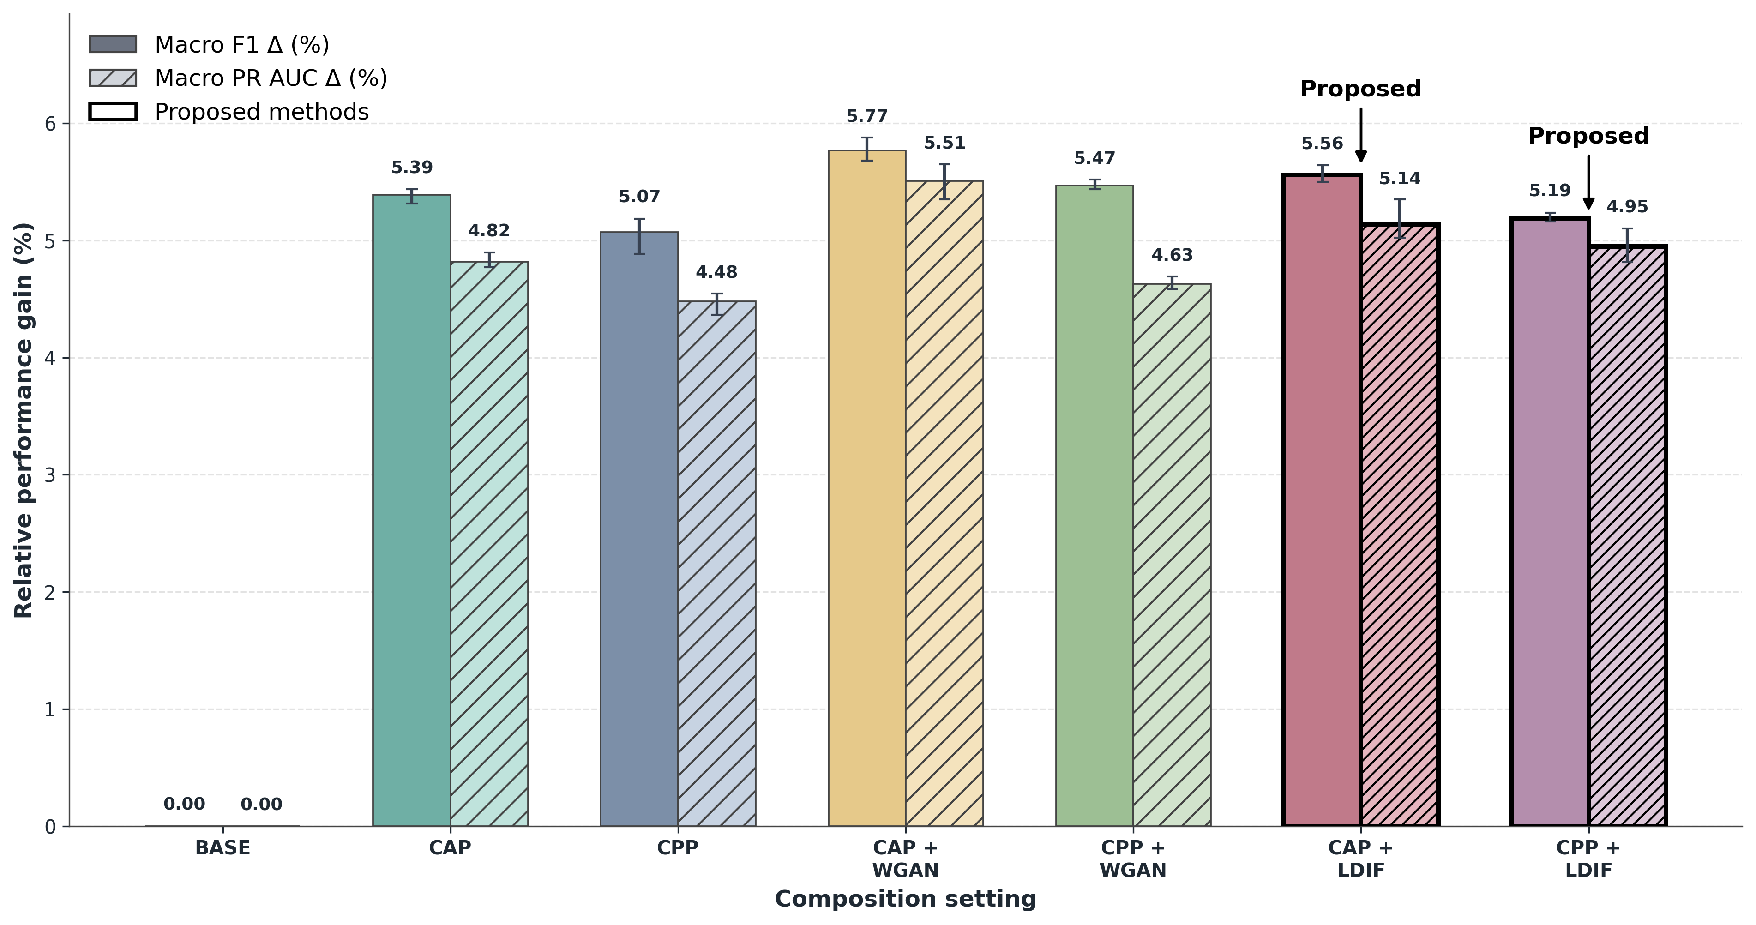
\includegraphics[width=1\textwidth]{images/augmentation_delta2.pdf}
    \caption{Relative performance gains (\%) of composition-based augmentation methods compared to the baseline, measured in Macro F1 (solid) and Macro PR AUC (hatched). The proposed methods are highlighted. Error bars indicate the min–max range across runs.}
    \label{fig:augmentation_delta2}
\end{figure}

Figure~\ref{fig:augmentation_delta} illustrates the effects of the combined methods by comparing the relative performance gains achieved using each method, and the narrow min-max range again shows the consistency of these gains.

While combinations including generative methods were able to further improve classification performance compared to CAP or CPP alone, the additional gains provided by these combinations were relatively modest.


\section{Additional Experiments}

The effectiveness of the proposed LDIF augmentation across different artifact classes is presented in Table~\ref{tab:combined_performance}. The results show improvements on all labels for both metrics. 

The highest improvement was achieved for the chew class with a +7.11\% gain in F1 score, while the models were also able to improve the classification of the elec label with gains of +3.42\% in F1 and +4.94\% in PR AUC. 

The proposed method could also achieve moderate improvement on the already well classified eyem label, reaching the highest F1 score of 0.8308 and the highest PR AUC of 0.7901, with gain of +2.59\% and +2.62\% respectively.

\begin{table}[H]
\centering

% ---------- F1 ----------
\begin{subtable}[t]{\textwidth}
\centering
\caption{F1 scores}
\renewcommand{\arraystretch}{1.2}
\setlength{\tabcolsep}{5pt}
\begin{tabular}{lccccc}
\hline
Setting & musc & eyem & elec & chew & Macro \\
\hline
BASE             & 0.7225 & 0.8098 & 0.7133 & 0.4880 & 0.6834 \\
LDIF         & 0.7438 & 0.8308 & 0.7377 & 0.5227 & 0.7087 \\
$\Delta$ (\%) & 2.94    & 2.59    & 3.42    & 7.11    & 3.70    \\
\hline
\end{tabular}
\end{subtable}

\vspace{0.4em}

% ---------- PR AUC ----------
\begin{subtable}[t]{\textwidth}
\centering
\caption{PR AUC scores}
\renewcommand{\arraystretch}{1.2}
\setlength{\tabcolsep}{5pt}
\begin{tabular}{lccccc}
\hline
Setting & musc & eyem & elec & chew & Macro \\
\hline
BASE             & 0.6397 & 0.7699 & 0.6310 & 0.5036 & 0.6360 \\
LDIF         & 0.6643 & 0.7901 & 0.6622 & 0.5166 & 0.6583 \\
$\Delta$ (\%) & 3.84    & 2.62    & 4.94    & 2.58    & 3.50    \\
\hline
\end{tabular}
\end{subtable}

\caption{Per-class comparison of baseline (BASE) and proposed (LDIF) performance, measured in (a) F1 and (b) PR AUC. The bottom row reports relative improvements (\%) of LDIF over the baseline.}
\label{tab:combined_performance}
\end{table}

Figure~\ref{fig:augmentation_delta3} highlights the relative performance gains across classes and shows the small variability across runs, which suggests stable and reproducible results. Together, these evaluation results provide an overview of the improvements achieved by the proposed generative augmentation technique, benefiting classification performance for both previously well classified and misclassified labels, improving overall performance across all artifacts. 
\newline

\begin{figure}[H]
\centering
    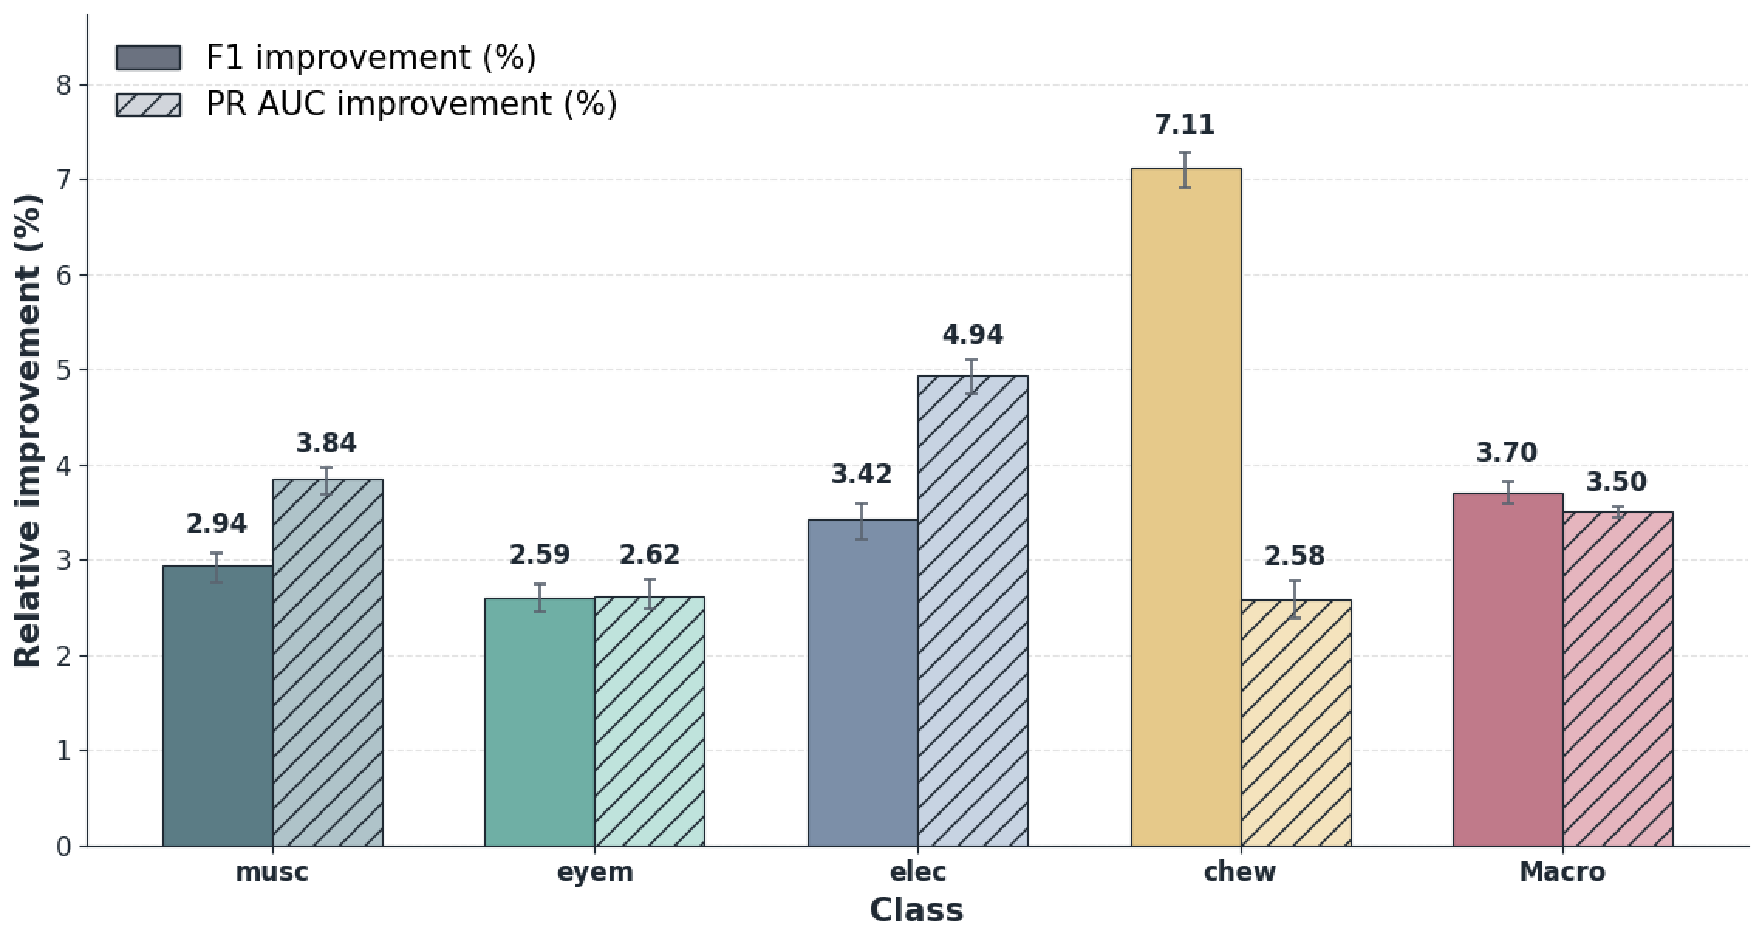
\includegraphics[width=0.9\textwidth]{images/augmentation_delta3.pdf}
    \caption{Relative improvement (\%) in classification performance across artifact classes, measured in F1 score (solid) and PR AUC (hatched). Error bars indicate the min–max range across runs.}
    \label{fig:augmentation_delta3}
\end{figure}

\chapter{Discussions}

\section{Effectiveness of the Proposed Method}

The proposed latent diffusion-based augmentation method proved to be effective in improving artifact classification performance. The main advantage of this method is its ability to generate realistic, high variance and fully synthetic EEG data rather than introducing small perturbations to existing data as in traditional augmentation techniques. Using this method to extend datasets allows better generalisation and reduces bias toward classes with larger number of datapoints, which is especially relevant for highly imbalanced datasets such as TUAR. 

Extending the set of underrepresented classes balances the overall data distribution, resulting in an increase in the number of training iterations that contain those labels and forcing the classification models to improve their ability to recognise these rare artifact patterns. Interestingly, a similar effect can be observed on classes with higher occurrence in the dataset, where the models also show smaller but consistent improvements in both metrics. The reason behind this behavior is that larger number of training datapoints allows the generative latent diffusion model to provide more realistic samples for dominant classes than for less frequent ones, allowing further improvement on overrepresented classes as well. 

In the context of artifact detection, it is highly positive that the proposed method was able to achieve improvements across all classes. This suggests that the method not only handles underrepresented and overrepresented classes well, but it is also able to generalise to statistically different EEG signal patterns. 

Conducting the diffusion process in a compressed latent space has the benefits of stability and efficiency. This dimensionality reduction results in more stable training compared to other generative models and allows the diffusion model to focus on the relevant information in the input EEG signals.

Overall, the results show that the proposed augmentation method is not only capable of improving EEG artifact classification but also helps overcome data scarcity and class imbalance, demonstrating performance gains in both evaluation metrics.

\section{Augmentation Method Comparison}

The proposed method achieved strong results compared to most other measured augmentations as well. In comparison with the nongenerative methods it outperformed all other augmentations except the segment recombination technique. These results were expected, because generative solutions proved to have stronger effect on performance in the past due to their robustness and ability to introduce significant variability into the dataset. 

Compared to the WGAN-based augmentation, the proposed method achieved similar gains in classification performance. While in some cases the addition of synthetic EEG windows generated by the latent diffusion model reached the highest score, for most models the WGAN-based method outperformed the proposed approach. 

The reason for this could be that diffusion-based approaches often require larger training datasets, while WGANs are able to converge using fewer samples and do not require learning a complex denoising process. Another likely factor is that during the data compression performed by the VAE, some temporal information is lost, which can be critical in case of EEG signals. Diffusion models are also harder to finetune, and if the sampling strategy or the noise scheduling mechanism is suboptimal, the quality of the generated EEG data can drop.

Two existing augmentation pipelines were combined with the proposed method and the WGAN-based generative augmentation. The synthetic EEG windows generated by the diffusion model were able to slightly improve upon the results originally achieved by the combined augmentations. Although the WGAN outperformed the latent diffusion again, the gains were relatively small compared to their standalone improvements over the baseline. The magnitude of the improvement can be explained by the nature of augmentation stacking, where combining augmentations may increase variance, benefitting generalisation, but also adds up the distortions making the datapoints less similar to real data. While too much augmentation can lead to underfitting, the introduction of the proposed augmentation proved to be advantageous by improving both metrics. 

The proposed method was not able to achieve the top score in either experiment, but introduced a generative technique capable of improving existing pipelines.

\section{Limitations}

One of the main limitations of the proposed generative augmentation method is that it requires a separate model for each artifact class. These models are not only trained separately, but for optimal performance separate hyperparameter optimisation are required. This makes it computationally expensive compared to other augmentations that achieve similar gains. 

Another limiting factor is the lack of validation step for the generated datapoints. Although the overall quality of the synthetic EEG windows is measured during the training of the diffusion model, when used, a filtering step could potentially improve the quality of the dataset extension.

While this method helped improve classification metrics on underrepresented major classes, the minor classes with even rarer occurrences are so scarce that the model is unable to learn and generate synthetic extensions. 

Information is potentially lost when the VAE constructs the latent representation of the input signal. While the compression benefits the diffusion process the lost temporal information may result in degraded quality and unrealistic EEG windows.

Another limitation is the dataset specificity. The method was only evaluated and optimised using the TUAR dataset, and while it contains the largest amount of annotated artifacts, testing on other datasets and possibly clinical validation are required to verify its performance in other settings.

\section{Future work}

\begin{description}

\item[\textbf{Generalisation and robustness.}] An important next step is the evaluation on other EEG artifact datasets. Cross-institution analysis using other TUAR versions (e.g., v2) and cross-dataset evaluation would provide information about generalisation potential and real world applicability.

\item[\textbf{Conditional diffusion model.}] Transforming the current method into conditional generation using a single diffusion model could help overcome the limitation of per-class training and optimisation. It would also help reduce the computational cost of both training and synthetic data generation.

\item[\textbf{Improved autoencoders architecture.}] Exploring more advanced models, such as hierarchical VAE or VQ-VAE could help reduce the amount of information lost during the compression. Further developing this part of the architecture has the potential to improve generated EEG signal quality and increase the performance of the proposed generative augmentation method.

\item[\textbf{Data quality evaluation.}] Future work could explore evaluation methods for synthetic EEG data. Investigating artifact specific metrics that describe the similarity of synthetic and real datapoints accurately and validating the generated EEG windows with the help of medical experts could help in further optimising the proposed method.

\end{description}
\chapter{Conclusions}

The purpose of this study was to investigate the effect of the proposed generative augmentation method on EEG artifact classification performance in a highly imbalanced setting provided by the TUAR dataset. The study introduced a latent diffusion-based augmentation technique, in which a separate model was trained for each artifact and synthetically generated EEG data were used for dataset extension. Two comprehensive experiments were conducted, one comparing standalone performance of existing and the proposed augmentations, and another for measuring the effect of the proposed technique when combined with existing pipelines.

The results of the first experiment showed that the latent diffusion-based augmentation was able to improve classification models by approximately 3.7\% in Macro F1 and 3.5\% in Macro PR AUC. The second experiment demonstrated that combining the existing augmentation pipelines with the proposed method achieved small but consistent improvements over their baseline performance. While both experiments demonstrated improved performance using the diffusion-based technique, the proposed augmentation was outperformed by both nongenerative and WGAN-based methods. 

The analysis of the results indicates that the proposed method is not yet able to match the performance of the simpler WGAN-based strategy. However, further optimising the information compression process and latent space representation within the VAE, the proposed model has the potential to achieve improved performance and outperform other generative augmentations.

In conclusion, the conducted experiments suggest that the proposed latent diffusion-based augmentation is a promising direction for enhancing artifact detection and handling imbalanced EEG datasets.


\cleardoublepage
\phantomsection
\addcontentsline{toc}{chapter}{\biblabel}
\printbibliography[title=\biblabel]

\appendix
\chapter{Appendix}

\section*{Resources and Links}

\begin{itemize}
    \item Dataset: \url{https://isip.piconepress.com/projects/nedc/html/tuh_eeg/}
    \item Braindecode: \url{https://braindecode.org/stable/index.html}
    \item GitHub: \url{https://github.com/BenjaminToth/MScThesis}
\end{itemize}

\section*{Example Synthetic EEG Artifact}

\begin{figure}[H]
\centering
    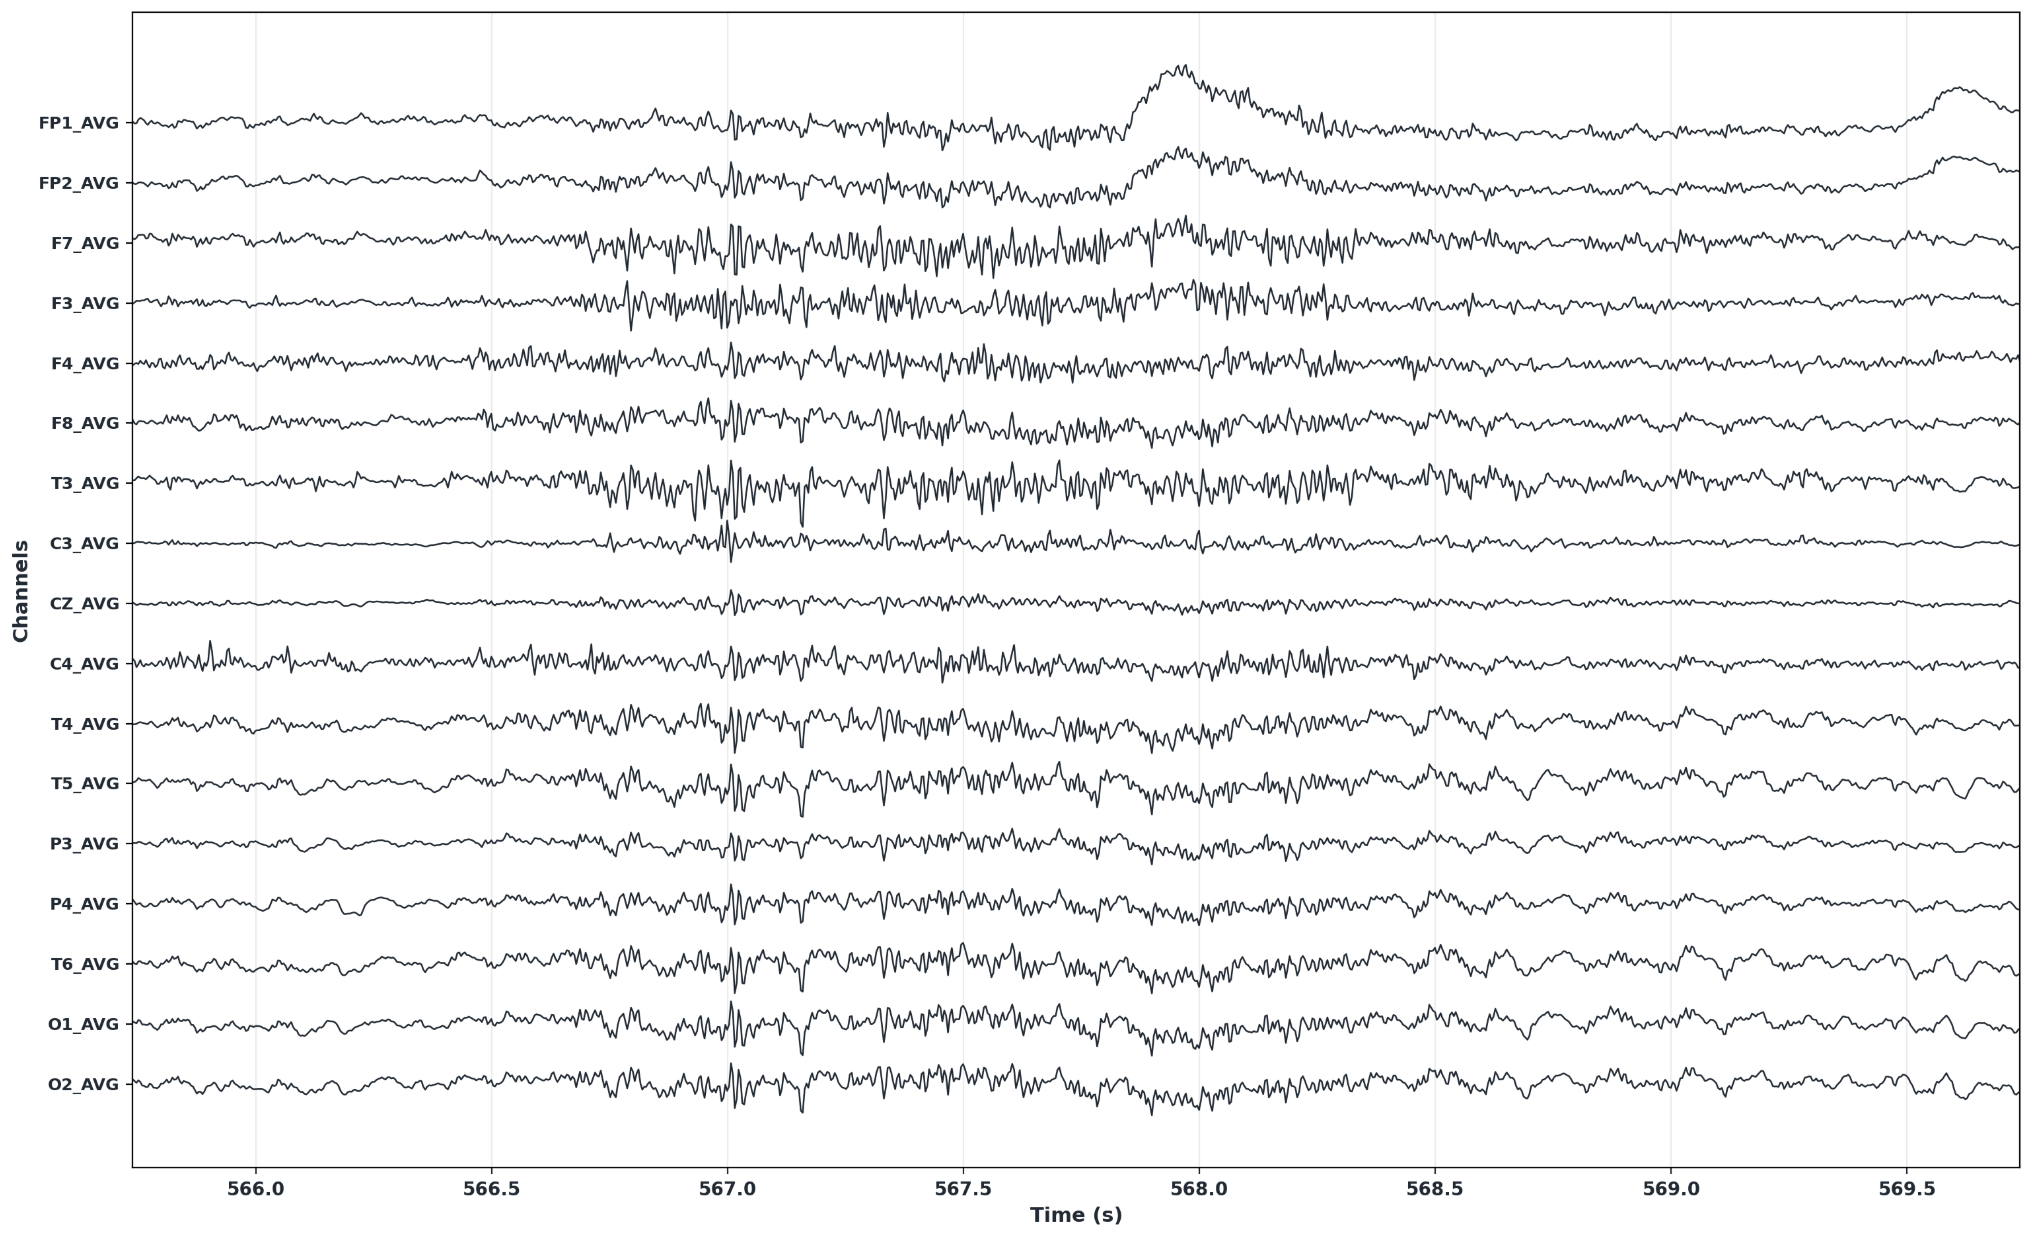
\includegraphics[width=1\textwidth]{images/synthetic_eyem.png}
    \caption{Example synthetic EEG window generated using the proposed latent diffusion-based augmentation method. For the generation the model corresponding to the eyem artifact was used.}
    \label{fig:eyem}
\end{figure}

\section*{Model Parameters}

The models are based on the original Braindecode implementation, with small modifications to better suit the requirements of this study.

All models were trained on EEG segments with $C=17$ channels and $T=2000$ time samples.

\paragraph{EEGNet}
\begin{itemize}
    \item Dropout $p=0.5$
    \item Kernel sizes: $k_t=63$, $k_d=15$
    \item Filters: $F_1=8$, depth multiplier $D=2$, $F_2=16$
\end{itemize}

\paragraph{EEGNeX}
\begin{itemize}
    \item Activation: ELU, dropout $p=0.5$
    \item Filters: $F_1=8$, $F_2=32$, $D=2$, $F_3=64$
    \item Kernel sizes: $k_{1,2}=32$, $k_4=16$, $k_5=16$
    \item Dilations: $d_4=2$, $d_5=4$
    \item Pooling: $p_4=4$, $p_5=8$
    \item Max-norm: conv $=1.0$, linear $=0.25$
\end{itemize}

\paragraph{EEGInceptionERP}
\begin{itemize}
    \item Activation: ELU, dropout $p=0.5$
    \item Base filters: $F=8$, depth multiplier $D=2$
    \item Stage 1 kernels: $(64, 32, 16)$
    \item Stage 2 kernels: $(16, 8, 4)$
    \item Stage 3--4 kernels: $k_3=8$, $k_4=4$
    \item Pooling: $p_1=4$, $p_2=2$, $p_3=2$, $p_4=2$
\end{itemize}

\paragraph{CNN-LSTM}
\begin{itemize}
    \item Activation: ELU, dropout $p=0.35$
    \item CNN filters: $F_1=64$, $F_2=128$
    \item Kernel sizes: $k_1=15$, $k_2=7$
    \item Pooling: $p_1=2$, $p_2=2$
    \item LSTM: hidden size $H=192$, layers $L=2$, bidirectional
\end{itemize}

\paragraph{EEGConformer}
\begin{itemize}
    \item Embedding size: $D=40$
    \item Temporal kernel: $k_t=25$
    \item Patch pooling: kernel $=75$, stride $=15$
    \item Transformer: depth $L=6$, heads $H=10$
    \item Feed-forward expansion: $4$
    \item Classification head: hidden size $256$
    \item Activations: ELU (front-end), GELU (transformer)
    \item Dropout: $p=0.5$, attention dropout $p_{\text{att}}=0.5$
\end{itemize}

\paragraph{WGAN-GP}
\begin{itemize}
    \item Input/output shape: $C=17$, $T=2000$
    \item Latent dimension: $z=128$
    \item Generator base channels: $256$
    \item Generator channel progression: $256 \rightarrow 256 \rightarrow 128 \rightarrow 64 \rightarrow 32 \rightarrow 17$
    \item Generator kernel sizes: $k=5$ (hidden), $k_{\text{out}}=7$
    \item Generator normalization: GroupNorm, activation: LeakyReLU$(0.2)$
    \item Critic channels: $64 \rightarrow 128 \rightarrow 256 \rightarrow 512$
    \item Critic kernel size: $k=5$, stride $s=2$, pooling length $16$
    \item Gradient penalty: $\lambda_{\mathrm{gp}}=10$
    \item Training ratio: $n_{\text{critic}}=5$
    \item Optimizer: Adam, $\mathrm{lr}_G=\mathrm{lr}_D=2 \times 10^{-4}$, $\beta_1=0.0$, $\beta_2=0.9$
\end{itemize}

\paragraph{Latent Diffusion Model}
\begin{itemize}
    \item Input/output shape: $C=17$, $T=2000$
    \item Latent shape: $C_z=32$, $T_z=125$
    \item VAE: base channels $F=128$, downsampling factor $16$, kernel sizes $k=5$ (encoder/decoder), $k_{\mathrm{out}}=7$, activation SiLU, GroupNorm
    \item Latent U-Net: base channels $F=128$, channel multipliers $(1,2,4)$, residual block kernel size $k=3$, downsampling kernel $k=4$ with stride $s=2$, bottleneck blocks $=2$
    \item Time embedding: sinusoidal, dimension $D_t=256$, MLP expansion $4\times$
    \item Diffusion: timesteps $N=1000$, beta schedule cosine, inference steps $50$
    \item Training: VAE epochs $10$, diffusion epochs $20$, batch size $32$, gradient clipping $1.0$
    \item Optimisation: Adam, $\mathrm{lr}_{\mathrm{VAE}}=10^{-3}$, $\mathrm{lr}_{\mathrm{diff}}=2 \times 10^{-4}$
    \item VAE objective: reconstruction loss $L_1$, KL weight $\lambda_{\mathrm{KL}}=10^{-4}$
    \item Latent scaling: auto-estimated to approximately unit variance
\end{itemize}

\newpage

\subsubsection{Use of AI Tools and Figure Attribution:}

All architecture images were created by the author.

AI tools were used to improve the grammar and vocabulary of most parts of this thesis in order to achieve an appropriate academic style. All AI-generated suggestions were carefully reviewed and either revised or discarded as necessary.

The code in the accompanying repository was developed with the assistance of AI tools. These tools were used for tasks such as error handling, visualisation, README refinement, implementation of helper functions, as well as code optimisation and refactoring. AI assistance also contributed to the fine-tuning of model architectures from braindecode. All AI-generated code and suggestions were carefully reviewed and, where necessary, modified or rejected by the author.

The preprocessing pipeline and data loaders were developed with the help of, and based on, the work of the AI Research Group at the Institute of Mathematics, Eötvös Loránd University.



\end{document}